%% \label{app:gwendolen}
%
\chapter{The \gwendolen\ Programming Language}
\label{chap:gwendolen}

This chapter contains a set of tutorials on the \gwendolen\ \index{Gwendolen} programming language.  The semantics of the language can be found in~\cite{dennis17gwen}.  These tutorials give an introduction to the use of the language.

\section{Tutorial 1 --- Introduction to Running Gwendolen Programs}\index{Gwendolen}

{
  \let\section\subsection
  \let\subsection\subsubsection
  \let\subsubsection\paragraph
  
  \label{tutorial:gwendolen:introduction}
This is the first in a series of tutorials on the use of the \gwendolen\ programming language\index{Gwendolen}.  This tutorial covers the basics of running \gwendolen\ programs\index{Gwendolen!running programs}, the configuration files\index{Gwendolen!configuration}, perform goals\index{goal!perform}\index{goal} and print actions\index{action}\index{action!print}.  It assumes the reader is familiar with the basics of \prolog\ notation.
Files for this tutorial can be found in the
\texttt{mcapl} distribution in the directory
\begin{quote}
\texttt{src/examples/gwendolen/tutorials/tutorial1}.
\end{quote}
%
The tutorials assume some familiarity with the \prolog\ programming language as well as the basics of running Java programs either at the command line or in Eclipse.

\section{Hello World}

You will find a \gwendolen\ program in the tutorial directory called \texttt{hello\_world.gwen}\index{example!hello\_world}\index{Gwendolen}.  It's contents should look like Example~\ref{code:hello_world}.
\begin{ourexample}
\label{code:hello_world}
\begin{lstlisting}[basicstyle=\footnotesize\sffamily,language=Gwendolen]
GWENDOLEN

:name: hello

:Initial Beliefs:

:Initial Goals:

say_hello [perform]

:Plans:

+!say_hello [perform] : {True} <- print(hello);
\end{lstlisting}
\end{ourexample}

This can be understood as follows\index{Gwendolen}.  Line 1 states the language in which the program is written (this is because the \ail\ allows us to create multi-agent systems from programs written in several different languages).  Line 3 gives the name of the agent (\lstinline{hello}).  Line 5 starts the section for initial beliefs (there are none).  Line 7 starts the section for initial goals.  There is one a \emph{perform} goal\index{goal}\index{goal!perform}\index{goal}\index{goal!perform}\index{goal}\index{goal!perform}\index{goal}\index{goal!perform} to \lstinline{say_hello} (we wi\index{plan}ll cover the different sorts of \index{plan}goal in a later tutorial).  Line\index{plan} 11 starts the section for plans\index{action}\index{action!print}x{plan}.  There is one plan which can be und\index{action}\index{action!print}erstood as saying if the goal is \index{plan!guard}to say hell\index{action}\index{action!print}o \lstinline{+!say_hello} then do\index{plan!guard} the action\index{action}\index{action!print} \lstinline{print(hello)}.  There\index{plan!guard} is a third component to the plan (\lstinline+{True}+) which is a \emph{guard}\index{plan!guard} that must be true before the plan is applied.  In this case the guard is always true so the plan applies whenever the agent has a goal to perform \lstinline{+!say_hello}.

\subsection{Running the Program}

To run the program\index{Gwendolen}\index{Gwendolen!running programs} you need to run the \java\ program \texttt{ail.mas.AIL}\index{AIL (class)} and supply it with a suitable configuration\index{Gwendolen!configuration}\index{configuration!gwendolen} file as an argument.  You will find an appropriate configuration file, \texttt{hello\_world.ail}\index{example!hello\_world} in the same directory as \texttt{hello\_world.gwen}.  You can do this either from the command line or using the Eclipse \texttt{run-AIL}\index{run-AIL} configuration (with \texttt{hellow\_world.ail} selected in the Package Explorer window) as detailed in the \mcapl\ manual.

Run the program now.

\section{The Configuration File}\index{Gwendolen}
Now open the configuration file, \texttt{hello\_world.ail}.\index{configuration!gwendolen}\index{Gwendolen!configuration}

\noindent\rule{\textwidth}{1pt}
\begin{verbatim}
mas.file = /src/examples/gwendolen/tutorials/tutorial1/hello_world.gwen
mas.builder = gwendolen.GwendolenMASBuilder

env = ail.mas.DefaultEnvironment

log.warning = ail.mas.DefaultEnvironment
\end{verbatim}
\rule{\textwidth}{1pt}

This is a very simple configuration consisting of four items only.
\begin{description}
\item[mas.file]\index{mas.file}\index{Gwendolen} gives the path to the \gwendolen\ program to be run.
\item[mas.builder]\index{mas.builder} gives a java class for building the file.  In this case \texttt{gwendolen.GwendolenMASBuilder}\index{GwendolenMASBuilder (class)} parses a file containing one or more \gwendolen\ agents and compiles them into a multi-agent system\index{multi-agent system}.
\item[env] provides an environment\index{environment} for the agent to run in.  In this case we use the default environment\index{environment!default}\index{DefaultEnvironment (class)} provided by the \ail.\index{AIL}
\item[log.warning]\index{logging} sets the level of output for the class \texttt{ail.mas.DefaultEnvironment}.  This is a pretty minimal level of output (warnings only).  We will see in later tutorials that it is often useful to get more output than this.
\end{description}

\section{Some Simple Exercise to Try}\index{Gwendolen!exercises}
\begin{enumerate}
\item Change the filename of \texttt{hello\_world.gwen} to something else (e.g., \texttt{hello.gwen}.  Update \texttt{hello\_world.ail} to reflect this change.  Check you can still run the program.
\item Edit the hello world program so it prints out \texttt{hi} instead of \texttt{hello}.
\item Edit the hello world program so the goal is called \texttt{hello} instead of \texttt{say\_hello}.  If you don't change the plan notice how the behaviour of the program changes.  Edit the plan to return to the original behaviour of the program.
\item Change the plan to
\begin{verbatim}
+!say_hello [perform] : {True} <- print(hello), print(louise);
\end{verbatim} and see how this changes the behaviour of the program.
\item Experiment getting the program to print out various different things.  Note that in order to print a string containing whitespace, the string must be contained in double quotes (i.e. \lstinline{print("hello world");})\index{example!hello\_world}\index{action!print!whitespace}\index{action!print}
\end{enumerate}


  }

\section{Tutorial 2 --- Simple Beliefs, Goals and Actions}\index{Gwendolen}

{
  \let\section\subsection
  \let\subsection\subsubsection
  \let\subsubsection\paragraph
  
  \label{tutorial:gwendolen:bda}
This is the second in a series of tutorials on the use of
the \gwendolen\ programming language\index{Gwendolen}.  This tutorial
covers the basics of beliefs\index{belief}, goals\index{goal} and
actions\index{action} as they appear in \gwendolen.

Files for this tutorial can be found in the \texttt{mcapl}
distribution in the directory
\begin{quote}
\texttt{src/examples/gwendolen/tutorials/tutorial2}.
\end{quote}

\section{Pick Up Rubble}

\begin{sloppypar}
You will find a \gwendolen\
program\index{Gwendolen}\index{example!pickuprubble} in the tutorial
directory called \texttt{pickuprubble.gwen}.  It's contents should
look like Example~\ref{code:pickuprubble}.
\end{sloppypar}
\begin{ourexample}
\label{code:pickuprubble}\quad \\
\begin{lstlisting}[basicstyle=\sffamily,language=Gwendolen,style=easslisting]
GWENDOLEN

:name: robot

:Initial Beliefs:

:Initial Goals:

goto55 [perform]

:Plans:

+!goto55 [perform] : {True} <- move_to(5, 5);

+rubble(5, 5): {True} <- lift_rubble;

+holding(rubble): {True} <- print(done);
\end{lstlisting}
\end{ourexample}
This is a program for moving around a simple grid based
environment\index{environment} and picking up rubble.  The robot can
perform three actions\index{action} in this
environment, \index{Gwendolen}\index{example!pickuprubble}
\begin{description}
\item[move\_to(X, Y)] moves to grid square (X, Y) and adds the belief\index{belief}\index{belief!add} \lstinline{at(X, Y)}.
\begin{sloppypar}
\item[lift\_rubble] attempts picks up a piece of rubble and adds the belief\index{belief}\index{belief!add} \lstinline{holding(rubble)} if there is rubble at the robot's location.
\end{sloppypar}
\item[drop] drops whatever the robot is holding and removes any beliefs\index{belief}\index{belief!remove} about what the robot is holding.
\end{description}
The default actions\index{action}\index{action!print}
(e.g., \lstinline{print}) are also available to the robot.  As the
environment\index{environment} is set up there is a block of rubble at
square (5, 5) which the robot will see if is in square (5, 5).  When
the robot picks something up it can see that it is holding it.  This
environment is programmed in \java\ and is the
class \lstinline{gwendolen.tutorials.SearchAndRescueEnv}\index{SearchAndRescueEnv
(class)}.

The program can be understood as follows.  \index{Gwendolen}
\begin{description}
\item[Line 1] states the language in which the program is written (this is because the \ail\ allows us to create multi-agent systems from programs written in several different languages).  \index{Gwendolen}
\item[Line 3] gives the name of the agent (\lstinline{robot}).  \index{Gwendolen!agent name}
\item[Line 5] starts the section for initial beliefs (there are none).  \index{belief}\index{belief!initial}
\item[Line 7] starts the section for initial goals.  There is one a \emph{perform} goal to \lstinline{goto55}.\index{goal}\index{goal!initial}
\item[Line 11] starts the section for plans\index{plan}.  There are
  three plans.  The first (line 13) states that in order to
  perform\index{goal}\index{goal!perform} \lstinline{goto55} the agent
  must move to square (5, 5).  The second (line 15) states that if the
  agent sees rubble at 5, 5 it should lift the rubble and the third
  (line 17) states that if the agent sees it is holding rubble then it
  should print done.\index{action}\index{action!print}
\end{description}

There are three different sorts of syntax being used here to
distinguish between beliefs, goals and
actions.\index{Gwendolen}\index{belief}\index{goal}\index{action}

\begin{description}
\item[Beliefs]\index{belief} Beliefs are predicates (e.g.,
  \lstinline{rubble(5, 5)} that are preceded either by a + symbol (to
  indicate a adding a belief\index{belief!add}) or a - symbol (to
  indicate removing a belief\index{belief!remove}).
\item[Goals]\index{goal} Goals are predicates preceded by an
  exclamation mark (e.g., \lstinline{!goto55}) again these are then
  preceded either by a + symbol (to indicate a adding a
  goal\index{goal!add}) or a - symbol (to indicate removing a
  goal\index{goal!remove}).  After the goal predicate there is also a
  label stating what kind of goal it is.  Goals can either be
  \emph{perform}\index{goal!perform} goals or
  \emph{achieve}\index{goal!achieve} goals.  We will discuss the
  difference between these in a moment.
\item[Actions]\index{action} Are just predicates.  Actions are
  performed externally to the agent and can not be added or removed
  (they are just done).
\end{description}

\subsection{Running the Program and Getting more Log output}\index{Gwendolen}\index{Gwendolen!running programs}

\begin{sloppypar}
To run the program you need to call \texttt{ail.mas.AIL}\index{AIL
  (class)} and supply it with a suitable configuration
file\index{configuration!gwendolen}\index{Gwendolen!configuration}.
You will find an appropriate configuration file,
\texttt{pickuprubble.ail}\index{example!pickuprubble} in the same
directory as \texttt{pickuprubble.gwen}.  You can do this either from
the command line or using the Eclipse \texttt{run-AIL}\index{run-AIL}
configuration as detailed in the \mcapl\ manual.
\end{sloppypar}

Run the program now.\index{Gwendolen}\index{Gwendolen!running programs}

As in Tutorial 1, all you see is the robot
printing\index{action}\index{action!print} the message
\lstinline{done} once it has finished.  However what has happened is
that the robot moved to square (5, 5) (because of the perform
goal\index{goal}\index{goal!perform}).  Once in square (5, 5) it saw
the rubble and so lifted it (thanks to the second plan\index{plan}).
Once it had lifted the rubble it saw that it was holding it and
printed \lstinline{done} (thanks to the third plan).

You can get more information about the execution of the program by
changing the logging information in the configuration file.  Open the
configuration file and
edit\index{Gwendolen}\index{logging}\index{Gwendolen!logging}\index{configuration!gwendolen}\index{Gwendolen!configuration}
\begin{verbatim}
log.warning = ail.mas.DefaultEnvironment
\end{verbatim}
to
\begin{verbatim}
log.info = ail.mas.DefaultEnvironment
\end{verbatim}
You will now see logging information printed out about each action the robots takes.\index{DefaultEnvironment (class)}

If you add the line
\begin{verbatim}
log.format = brief
\end{verbatim}
to the configuration file you will get the log messages in a briefer form.\index{log.format}\index{Gwendolen}\index{Gwendolen!configuration}\index{configuration!gwendolen}

\section{Perform and Achieve Goals}\index{Gwendolen}\index{goal}\index{goal!perform}\index{goal!achieve}
\lstinline{pickuprubble_achieve.gwen} is a slightly more complex
version of the rubble lifting program which introduces some new
concepts.  It is shown in
Example~\ref{code:pickuprubble_achieve}\index{example!pickuprubble}
\begin{figure}[htb]
\begin{ourexample}
\label{code:pickuprubble_achieve} \quad \\
\begin{lstlisting}[basicstyle=\sffamily,style=easslisting,language=Gwendolen]
GWENDOLEN

:name: robot

:Initial Beliefs:

possible_rubble(1, 1)
possible_rubble(3, 3)
possible_rubble(5, 5)

:Initial Goals:

holding(rubble) [achieve]

:Plans:

+!holding(rubble) [achieve] : 
  {B possible_rubble(X, Y), ~B no_rubble(X, Y)} <- move_to(X, Y);

+at(X, Y) : {~B rubble(X, Y)} <- +no_rubble(X, Y);

+rubble(X, Y): {B at(X, Y)} <- lift_rubble;

+holding(rubble): {True} <- print(done);
\end{lstlisting}
\end{ourexample}
\end{figure}
The first changes are in lines 7-9.  Here we have a list of initial
beliefs\index{belief}\index{belief!initial}.  The agent believes there
may be rubble in one of three squares (1, 1), (3, 3) and (5, 5).  As
we know, in the environment, there is only rubble in (5,
5).\index{environment}

The next change is in line 13.  Here instead of a \emph{perform}
goal\index{goal}\index{goal!perform}, \lstinline{goto55 [perform]}
there is an \emph{achieve} goal\index{goal!achieve},
\lstinline{holding(rubble) [achieve]}.  The difference between perform
goals and achieve goals is as follows:
\begin{itemize}
\item When an agent adds a perform goal it searches for a plan for
  that goal, executes the plan and then drops the goal, it does not
  check that the plan has succeeded.\index{goal!perform}
\item When an agent adds an achieve goal it searches for a plan for
  that goal, executes the plan and then checks to see if it now has a
  belief corresponding to the goal.  If it has no such beliefs it
  searches for a plan again, if it does have such a belief then it
  drops the goal.\index{goal!achieve}
\end{itemize}
In the case of this program the robot will continue executing the plan
for \lstinline{holding(rubble)} until it actually believes that it is
holding some rubble.\index{belief}

On lines 17 and 18, you can see the plan\index{plan} for the
goal\index{goal}.  This plan no longer has a trivial
guard\index{plan!guard}.  Instead the plan only applies if the agent
believes\index{belief} that there is possible rubble in some square
(X, Y) and it does not (the $\sim$ symbol) believe\index{belief!not
  believe} there is no rubble in that square.  If it can find such a
square then the robot moves\index{action} to it.  The idea is that the
robot will check each of the possible rubble squares in turn until it
successfully finds and lifts some rubble.  Note that we are using
capital letters for variables\index{Gwendolen!variables} that can be
unified against beliefs (like in \prolog).

The plan\index{plan} at line 20 gets the robot to add the
belief\index{belief} \lstinline{no_rubble(X, Y)} if it is at some
square, (X, Y), and it can't see any rubble there.  By this means the
plan in lines 17 and 18 will be forced to pick a different square next
time it executes.  Up until now all the plans you have used have
simply executed actions in the plan body.  This one adds a
belief.\index{Gwendolen}

The plan at line 22 is similar to the plan in line 15 of
Example~\ref{code:pickuprubble} only in this case we are using
variables for the rubble coordinates rather than giving it the
coordinates (5, 5).\index{Gwendolen}\index{example!pickuprubble}

You can run this program using the \lstinline{pickuprubble_achieve.ail} configuration file.\index{Gwendolen}

\section{Some Simple Exercise to Try}\index{Gwendolen!exercises}
\begin{enumerate}
\item Instead of having the robot print \lstinline{done} once it has
  the rubble, get it to move to square (2, 2) and drop the rubble.

Hint: you may find you need to add a ``housekeeping'' belief that the
rubble has been moved to prevent the robot immediately picking up the
rubble once it has been dropped.
\item Rewrite the program so that instead of starting with an
  achievement goal \lstinline{holding(rubble)}, it starts with an
  achievement goal \lstinline{rubble(2, 2)} -- i.e., it wants to
  believe there is rubble in square (2, 2).

Hint: you may want to reuse the plan for achieve
\lstinline{holding(rubble)} by setting it up as a
subgoal\index{goal}\index{goal!subgoal}.  You can use this by adding
the command \lstinline{+!holding(rubble) [achieve]} in the body of a
plan.
\end{enumerate}
\begin{sloppypar}
Sample answers for these two exercises can be found in \texttt{gwendolen/examples/tutorials/tutorial2/answers}.
\end{sloppypar}



  }

\section{Tutorial 3 --- Plan Guards and Reasoning Rules}\index{Gwendolen}

{
  \let\section\subsection
  \let\subsection\subsubsection
  \let\subsubsection\paragraph
  
  
This is the third in a series of tutorials on the use of the \eass\ variant of the \gwendolen\ language.  This tutorial covers verifying \eass\ reasoning engines as described in~\cite{dennis14:_pract,DBLP:journals/cacm/FisherDW13}.\index{EASS}\index{autonomous systems}\index{autonomous systems!verification}\index{reasoning engine}

Files for this tutorial can be found in the \texttt{mcapl} distribution in the directory 
\begin{quote}
\texttt{src/examples/eass/tutorials/tutorial3}.
\end{quote}

The tutorial assumes a good working knowledge of Java programming.  It also assumes the reader is familiar with the basics of using \ajpf\ to verify programs (see \ajpf\ Tutorials 1 and 2).

\section{Overview}\index{autonomous systems!verification}\index{reasoning engine}
The process for verifying an \eass\ reasoning engine\index{reasoning engine} is to first analyse the agent program in order to identify all the shared beliefs\index{belief!shared} that are sent from the abstraction engine\index{abstraction engine}\index{EASS} to the reasoning engine.  In multi-agent systems\index{multi-agent system} it is also necessary to identify all messages\index{message} that the reasoning engine may receive from other agents in the environment.  This is discussed in some detail in~\cite{dennis14:_pract}.  Once a list of shared beliefs and messages has been identified, an environment\index{environment} is constructed for the reasoning engine alone in such a way that every time the agent takes an action the set of perceptions and messages available to it are created \emph{at random}\index{environment!random}\index{environment!for verifying autonomous systems}.  When model checking\index{model checking} the random selection causes the search tree\index{model checking!search tree} to branch and the model checker to explore all possibilities.

\section{Example}\index{example!motorway}
As an example we will consider the accelerating car controller we looked at in \eass\ tutorial 1.  The full code for this is show in Example~\ref{code:EASSverifexample} and from this we can see there are two shared beliefs\index{EASS}\index{belief!shared} used by the program, \lstinline{start} and \lstinline{at_speed_limit}.

\begin{ourexample}
\label{code:EASSverifexample} \quad \\
\begin{lstlisting}[basicstyle=\sffamily,style=easslisting,language=Gwendolen]
EASS

:abstraction: car

:Initial Beliefs:

speed_limit(5)
													
:Initial Goals:
		

:Plans: 
/* Default plans for handling messages */
+.received(:tell, B): {True} <- +B;   
+.received(:perform, G): {True} <- +!G [perform];
+.received(:achieve, G): {True} <- +!G [achieve];

+started : {True} <-
	assert_shared(start);

+yspeed(X) : {B speed_limit(SL), SL < X} <-
	assert_shared(at_speed_limit);
+yspeed(X) : {B speed_limit(SL), X < SL} <-
	remove_shared(at_speed_limit);
	
+! accelerate [perform] : {B yspeed(X)} <- accelerate;
+! accelerate [perform] : {~B yspeed(X)} <- print("Waiting for Simulator to Start");
+! maintain_speed [perform] : {True} <- maintain_speed;

:name: car
			
:Initial Beliefs:
													
:Initial Goals:
		
:Plans: 

+start: {True} <-
	+!at_speed_limit[achieve];

+! at_speed_limit [achieve] : {True} <-
	perf(accelerate),
	*at_speed_limit;

+at_speed_limit: {True} <-
	perf(maintain_speed);
\end{lstlisting} 
\end{ourexample}
\index{autonomous systems!verification}\index{reasoning engine}

For verification purposes, we are only interested in the reasoning engine\index{reasoning engine}\index{EASS} so we create a file containing just the reasoning engine.  This is \texttt{car\_re.eass} in the tutorial directory.  You will also find an \ail\ configuration file \texttt{car.ail}, a \jpf\ configuration file, \texttt{car.jpf} and a property specification file, \texttt{car.psl} in the tutorial directory.\index{autonomous systems!verification}\index{reasoning engine}

\begin{ourexample}\index{EASSVerificationEnvironment (class)}\index{example!motorway}\index{autonomous systems!verification}\index{reasoning engine}
\label{code:EASSverifenvironment} \quad \\
\begin{lstlisting}[basicstyle=\sffamily,style=easslisting,language=Java]
/**
 * An environment for verifying a simple car reasoning engine.
 * @author louiseadennis
 *
 */
public class VerificationEnvironment extends 
                       EASSVerificationEnvironment {
			
  public String logname = "eass.tutorials.tutorial3.VerificationEnvironment";
	
  public Set<Predicate> generate_sharedbeliefs() {
    TreeSet<Predicate> percepts = new TreeSet<Predicate>();
    boolean assert_at_speed_limit = random_bool_generator.nextBoolean();
    if (assert_at_speed_limit) {
      percepts.add(new Predicate("at_speed_limit"));
      AJPFLogger.info(logname, "At the Speed Limit");
    } else {
      AJPFLogger.info(logname, "Not At Speed Limit");
    }
		
    boolean assert_start = random_bool_generator.nextBoolean();
    if (assert_start) {
      percepts.add(new Predicate("start"));
      AJPFLogger.info(logname, "Asserting start");
    } else {
      AJPFLogger.info(logname, "Not asserting start");
    }
    return percepts;
  }
	
  public Set<Message> generate_messages() {
    TreeSet<Message> messages = new TreeSet<Message>();
      return messages;
  };
}
\end{lstlisting}
\end{ourexample}
\begin{sloppypar}
The environment\index{environment}\index{EASS} for verifying the car reasoning engine is shown in example~\ref{code:EASSverifenvironment}.  This subclasses \texttt{eass.mas.verification.EASSVerificationEnvironment} which sets up a basic environment for handling verification of single reasoning engines\index{reasoning engine}.  In order to use this environment you have to implement two methods, \texttt{generate\_sharedbeliefs()}\index{EASSVerificationEnvironment (class)!generate\_sharedbeliefs} and \texttt{generate\_messages()}\index{EASSVerificationEnvironment (class)!generate\_messages}.  It is assumed that these methods will randomly generate the shared beliefs and messages of interest to your application.  \texttt{EASSVerificationEnvironment} handles the calling of these methods each time the reasoning engine takes an action\index{action}.  It should be noted that \texttt{EASSVerificationEnvironment} ignores \lstinline{assert_shared} and \lstinline{remove_shared} actions, assuming these take negligible time to execute -- this is largely in order to keep search spaces\index{search space} as small as possible.\index{autonomous systems!verification}\index{reasoning engine}
\end{sloppypar}

In the example verification environment\index{EASS}, \texttt{generate\_messages}\index{EASSVerificationEnvironment (class)!generate\_messages}\index{EASSVerificationEnvironment (class)} returns an empty set of messages because we didn't identify any messages in the program.  \texttt{generate\_sharedbeliefs}\index{EASSVerificationEnvironment (class)!generate\_sharedbeliefs} is responsible for asserting \lstinline{at_speed_limit} and \lstinline{start}.  \texttt{EASSVerificationEnvironment} provides \texttt{random\_bool\_generator}\index{EASSVerificationEnvironment (class)!random\_bool\_generator} which is a member of the \texttt{ajpf.util.choice.UniformBoolChoice}\index{UniformBoolChoice (class)} class and \texttt{random\_int\_generator}\index{EASSVerificationEnvironment (class)!random\_int\_generatpr} which is a member of the \texttt{ajpf.util.choice.UniformIntChoice}\index{UniformIntChoice (class)} class.  These can be used to generate random boolean and integer values.  In this case \texttt{random\_bool\_generator} is being used to generate two booleans, \texttt{assert\_at\_speed\_limit} and \texttt{assert\_start}.  If these booleans are true then the relevant predicate is added to the set returned by the method while, if it is false, nothing is added to the set.  An \texttt{AJPFLogger}\index{AJPFLogger (class)} is used to print out whether the shared belief was generated or not -- this can be useful when debugging failed model checking runs.\index{debugging}\index{debugging!model checking}\index{autonomous systems!verification}\index{reasoning engine}

There are four properties in the property specification file:
\begin{description}
\item[1] $\always \neg \lbelief{\texttt{car}}{crash}$ -- The car never believes it has crashed.  We know this to be impossible -- no such belief is ever asserted -- but it can be useful to have a simple property like this in a file in order to check the basics of the model checking is working.
\item[2] $\always ( \lactions{\texttt{car}}{\mathit{perf}(accelerate)} \Rightarrow (\sometime \lactions{\texttt{car}}{\mathit{perf}(maintain\_speed)} \lor \always  \neg \lbelief{\texttt{car}}{at\_speed\_limit}))$ -- If the car ever accelerates then either eventually it maintains its speed, or it never believes it has reached the speed limit.
\item[3] $\always ( \lbelief{\texttt{car}}{at\_speed\_limit}) \Rightarrow \sometime \lactions{\texttt{car}}{\mathit{perf}(maintain\_speed)}$ -- If the car believes it is at the speed limit then eventually it maintains its speed.  Properties of this form are often not true because $\lactions{ag}{a}$ only applies to the last action performed and beliefs are often more persistent than that so the agent acquires the belief, $b$, does action $a$, and then does something else.  At this point it still believes $b$ but unless it does $a$ again the property will be false in LTL.  In this case, however, the property is true because \lstinline{perf(maintain_speed)} is the last action performed by the agent.
\item[4] $\always \neg \lbelief{\texttt{car}}{start} \Rightarrow \always \neg \lactions{\texttt{car}}{\mathit{perf}(accelerate)}$ -- If the car never believes the simulation has started then it never accelerates.
\end{description}  \index{property}\index{autonomous systems!verification}\index{reasoning engine}

The \jpf\ configuration file in the tutorial directory is set to check property 3.  It is mostly a standard configuration, as discussed in \ajpf\ tutorial 2.  However it is worth looking at the list of classes passed to \texttt{log.info}.  These are:\index{logging}\index{model checking}
\begin{description}
\item[ail.mas.DefaultEnvironment] As discussed in \ajpf\ tutorial 2, this prints out the actions that an agent has performed and is useful for debugging.\index{DefaultEnvironment (class)}
\begin{sloppypar}
\item[eass.mas.verification.EASSVerificationEnvironment]\index{EASSVerificationEnvironment (class)} This prints out when an agent is just about to perform an action, before all the random shared beliefs and messages are generated.  If both this class and \texttt{ail.mas.DefaultEnvironment} are passed to \texttt{log.info} then you will see a message before the agent does an action, then the search space branching as the random shared beliefs and messages are generated and then a message when the action completes.  You may prefer to have only one of these print out.
\end{sloppypar}
\item[eass.tutorials.tutorial3.VerificationEnvironment] As can be seen in example~\ref{code:EASSverifenvironment} this will cause information about the random branching to get printed.
\item[ajpf.product.Product] As discussed in \ajpf\ tutorial 2, this prints out the current path through the \ajpf\ search space.\index{Product (class)}
\end{description}\index{autonomous systems!verification}\index{reasoning engine}

\section{Messages}\index{message}\index{EASS}
Normally there is no need to construct messages in environments since this is handled by the way \texttt{ail.mas.DefaultEnvironment} handles send actions.  However for \eass\ verification environments, where messages must be constructed at random, it is necessary to do this in the environment.\index{autonomous systems!verification}\index{reasoning engine}

The important class is \texttt{ail.syntax.Message} and the main constructor of interest is \texttt{public Message(int ilf, String s, String r, Term c)}.  The four parameters are\index{Message (class)}
\begin{description}
\item[ilf] This is the \emph{illocutionary force} or the \emph{performative}.  For \eass\ agents this should be 1, for a tell message, 2 for a perform message and 3 for an achieve message.  If in doubt you can use the static fields \texttt{EASSAgent.TELL}, \texttt{EASSAgent.PERFORM} and \texttt{EASSAgent.ACHIEVE}.\index{performative}\index{EASSAgent (class)}\index{EASSAgent (class)!TELL}\index{EASSAgent (class)!PERFORM}\index{EASSAgent (class)!ACHIEVE}.
\item[s] This is a string which is the name of the sender of the message.\index{message!sender}
\item[r] This is a string which is the name of the receiver of the message.\index{message!recipient}
\item[c] This is a term for the content of the message and should be created using the \ail\ classes for \texttt{Predicate}s etc.\index{message!logical content}\index{Predicate (class)}
\end{description}\index{autonomous systems!verification}\index{reasoning engine}

Where messages are to be randomly generated a list of them should be created in \texttt{generate\_messages}.\index{EASSVerificationEnvironment (class)!generate\_messages}

\section{Exercises}\index{EASS!exercises}\index{autonomous systems!verification}\index{reasoning engine}

\subsection{Exercise 1}
Take the sample answer for exercise 2 in \eass\ tutorial 1, and verify that if the car never gets an alert then it never stops.  As usual you can find a sample answer in the \texttt{answers} sub-directory.

\subsection{Exercise 2}
In the tutorial directory you will find a reasoning engine, \texttt{car\_re\_messages.eass}.  This is identical to \texttt{car\_re.eass} apart from the fact that it can process tell messages.  Provide a verification environment where instead of \lstinline{start} being asserted as a shared belief, the agent receives it as a tell message from the simulator.  Check you can verify the same properties of the agent.  As usual you can find a sample answer in the \texttt{answers} sub-directory.



  }

\section{Tutorial 4 --- Troubleshooting}\index{Gwendolen}

{
  \let\section\subsection
  \let\subsection\subsubsection
  \let\subsubsection\paragraph
  
  \label{tutorial:gwendolen:debugging}
This is the fourth in a series of tutorials on the use of the
\gwendolen\ programming language.  This tutorial looks at some of the
things that typically cause errors in \gwendolen\ programs and how to
identify and fix the
errors.\index{Gwendolen}\index{Gwendolen!debugging}\index{debugging}\index{debugging!Gwendolen} 

For this tutorial we will be working with files from previous
tutorials but editing them to introduce errors.  You may wish to
create a separate folder, \texttt{tutorial4} for this work and copy
files into it.  Remember to update the paths in your configuration
files if you do so. 

\gwendolen\ does not have its own debugger, however you can get a long
way using error outputs and logging information.\index{logging} 

\section{Path Errors}\index{debugging!could not find file}\index{Gwendolen}
If you supply the wrong path or filename in a
configuration\index{Gwendolen!configuration}\index{configuration!gwendolen}
file \gwendolen\ will not be able to find the program you want to run.
You will see an error similar to the following:  
\begin{verbatim}
ail.mas.AIL[SEVERE|main|3:24:57]: Could not find file.  Checked: 
 /src/examples/gwendolen/tutorials/tutorial3/pickuprubble_achiev.gwen,
 /Users/lad/src/examples/gwendolen/tutorials/tutorial3/pickuprubble_achiev.gwen,
 /Users/lad/Eclipse/mcapl/src/examples/gwendolen/tutorials/tutorial3/pickuprubble_achiev.gwen 
\end{verbatim}

\gwendolen\ looks for program files on\index{Gwendolen}
\begin{enumerate}
\item The absolute path given in the configuration file --
  \index{configuration!gwendolen}\index{Gwendolen!configuration} 

\texttt{/src/examples/gwendolen/tutorials/tutorial3/pickuprubble\_achiev.gwen}
above. 
\item The path from the \texttt{HOME} environment variable (normally the user's home directory on Unix systems) -- 

\texttt{/Users/lad/src/examples/gwendolen/tutorials/tutorial3/pickuprubble\_achiev.gwen} above.
\item The path from the directory from which the \java\ program
  \texttt{ail.mas.AIL} is called  -- \index{AIL (class)} 

\texttt{/Users/lad/Eclipse/mcapl/src/examples/gwendolen/tutorials/tutorial3/pickuprubble\_achiev.gwen}
above. 
\item and the path from \texttt{AJPF\_HOME}\index{AJPF\_HOME} if that
  environment variable has been set -- not shown above. 
\end{enumerate}

These should provide sufficient information to appropriately correct
the path name. 

\section{Parsing Errors}\index{Gwendolen}\index{Gwendolen!parsing error}

Parsing errors typically arise because of failures to punctuate your
program correctly.  E.g., failing to close brackets, missing out
commas or semi-colons etc. 

This is the output that arises if you remove the comma between
\lstinline{possible_rubble(X, Y)} and \lstinline{~no_rubble(X, Y)} in
\texttt{pickuprubble\_achieve.gwen} from Tutorial 3.\index{mismatched
  input} 

\begin{verbatim}
line 36:47 mismatched input '~' expecting SEMI
java.lang.NullPointerException
	at ail.syntax.ast.Abstract_Rule.toMCAPL(Abstract_Rule.java:108)
	at gwendolen.syntax.ast.Abstract_GwendolenAgent.addStructures(Abstract_GwendolenAgent.java:90)
	at gwendolen.syntax.ast.Abstract_GwendolenAgent.toMCAPL(Abstract_GwendolenAgent.java:77)
	at gwendolen.syntax.ast.Abstract_GwendolenAgent.toMCAPL(Abstract_GwendolenAgent.java:48)
	at ail.syntax.ast.Abstract_MAS.toMCAPL(Abstract_MAS.java:117)
	at gwendolen.GwendolenMASBuilder.getMAS(GwendolenMASBuilder.java:95)
	at ail.mas.AIL.buildMAS(AIL.java:117)
	at ail.mas.AIL.AILSetup(AIL.java:80)
	at ail.mas.AIL.runAIL(AIL.java:61)
	at ail.mas.AIL.main(AIL.java:49)
ail.mas.AIL[SEVERE|main|3:15:19]: null 
\end{verbatim}

The first line of this output is from the parser.  This identifies the
line number (36) and character in the line (47) where the error was
first noticed.  It highlights the character that has caused the
problem, \texttt{\~} and then makes a guess at what it should have
been.  In this case the guess is incorrect.  It suggests a semi-colon,
\texttt{SEMI}, when a comma is needed.  This first line is frequently
the most useful piece of output for parsing
errors.\index{Gwendolen}\index{mismatched input} 

We then have a \java\ stack trace because, in this case, the parse
error has caused the whole problem to fail.  At the end is a log
message from the \java\ class \texttt{ail.mas.AIL}.\index{Gwendolen} 

It should be noted that parsing errors do not always cause the program
to crash.  For instance, if we delete the comma from between
\texttt{X} and \texttt{Y} in the guard of the first plan of this
program we get the following output:\index{Gwendolen} 

\begin{verbatim}
line 44:51 extraneous input 'Y' expecting CLOSE
ail.semantics.operationalrules.GenerateApplicablePlansEmptyProblemGoal[WARNING|main|3:19:44]: 
Warning no applicable plan for goal _aholding(rubble)() 
\end{verbatim}

In this case we once again get some useful output from the parser
giving us the line and position in the line where the error occurred.
It is followed by a warning that no plan can be found to match the
goal \texttt{holding(rubble)}.  That is because this is the plan that
didn't parse.\index{no applicable plan} 

\subsection{Some
  Exercises}\index{Gwendolen!debugging!exercises}\index{debugging!Gwendolen} 
Experiment with adding and deleting syntax from your existing
programming files and get used to the kinds of parsing errors that
they generate.  Remember that where a \texttt{no applicable plan}
warning is generated you will often need to manually stop the program
execution.\index{no applicable plan} 

\section{Why isn't my plan applicable?}\index{no applicable plan}\index{Gwendolen}

As mentioned \intutorial{\gwendolen}{3}{tutorial:gwendolen:guards}
sometimes a plan can fail because the agent has not had time to
process incoming beliefs and perceptions.  We can get more information
about the agent's operation by using log
messages.\index{logging}\index{Gwendolen!logging} 

Add the line
\begin{verbatim}
log.fine = ail.semantics.AILAgent
\end{verbatim}
to the configuration file for the sample solution to the second exercise \exercise{6}{\gwendolen}{3}{ex:tutorial3}.  This is in
\begin{quote}
\texttt{/src/examples/gwendolen/tutorials/tutorial3/answers/pickuprubble\_ex5.2.ail}
\end{quote}
This generates a lot of output.  If you are using Eclipse you may need
to set Console output to unlimited in Eclipse $\rightarrow$
Preferences $\rightarrow$ Run/Debug $\rightarrow$
Console.\index{Gwendolen}\index{example!pickuprubble}\index{AILAgent
  (class)} 

The output should start
\begin{verbatim}
ail.semantics.AILAgent[FINE|main|4:03:27]: Applying Perceive 
ail.semantics.AILAgent[FINE|main|4:03:27]: robot
=============
After Stage StageE :
[square/2-square(1,1), square(1,2), square(1,3), square(1,4), square(1,5), 
square(2,1), square(2,2), square(2,3), square(2,4), square(2,5), 
square(3,1), square(3,2), square(3,3), square(3,4), square(3,5), 
square(4,1), square(4,2), square(4,3), square(4,4), square(4,5), 
square(5,1), square(5,2), square(5,3), square(5,4), square(5,5), ]
[]
[]
source(self):: 
   *  start||True||+!_aall_squares_checked()()||[]
[] 
\end{verbatim}
This tells us that the agent is applying the rule from the agent's
\emph{reasoning cycle}\index{reasoning cycle} called
\texttt{Percieve}\index{Percieve (rule)} (we will discuss the
reasoning cycle in a later tutorial). 

Then we get the current state of the agent.  It is called,
\texttt{robot}, and we have a list of its beliefs\index{belief} (lots
of beliefs about squares), then a list of goals\index{goal} (none at
the start because it hasn't yet added the initial
goal\index{goal!initial}) and then a list of sent
messages\index{communication}\index{message}\index{message!sent} (also
empty) and then the intentions\index{intention}.  In this case the
initial intention is the \texttt{start}
intention\index{intention!start} and the intention is to acquire the
goal \texttt{all\_squares\_checked} which is an achievement goal (the
\texttt{\_a} at the start of the goal name) -- again we will cover
intentions in a later tutorial.\index{Gwendolen} 

A little further on in the output the agent adds this as a goal:
\begin{verbatim}
ail.semantics.AILAgent[FINE|main|4:10:45]: Applying Handle Add Achieve Test Goal with Event 
ail.semantics.AILAgent[FINE|main|4:10:45]: robot
=============
After Stage StageD :
[square/2-square(1,1), square(1,2), square(1,3), square(1,4), square(1,5), square(2,1), square(2,2), square(2,3), square(2,4), square(2,5), square(3,1), square(3,2), square(3,3), square(3,4), square(3,5), square(4,1), square(4,2), square(4,3), square(4,4), square(4,5), square(5,1), square(5,2), square(5,3), square(5,4), square(5,5), ]
[all_squares_checked/0-[_aall_squares_checked()]]
[]
source(self):: 
   *  +!_aall_squares_checked()||True||npy()||[]
   *  start||True||+!_aall_squares_checked()()||[]
[] 
\end{verbatim}
So you can see that \texttt{all\_squares\_checked} now appears as a goal in the goal list. \index{Gwendolen}

\begin{sloppypar}
If you remove the action \texttt{do\_nothing} from the first plan\ in
\texttt{pickuprubble\_ex5.2.gwen}\index{example!pickuprubble} then you
end up with repeating output of the form: 
\end{sloppypar}

\begin{verbatim}
ail.semantics.AILAgent[FINE|main|4:20:16]: Applying Generate Applicable Plans Empty with Problem Goal 
ail.semantics.AILAgent[FINE|main|4:20:16]: robot
=============
After Stage StageB :
[at/2-at(5,5), , 
checked/2-checked(1,1), checked(1,2), checked(1,3), checked(1,4), checked(1,5), checked(2,1), checked(2,2), checked(2,3), checked(2,4), checked(2,5), checked(3,1), checked(3,2), checked(3,3), checked(3,4), checked(3,5), checked(4,1), checked(4,2), checked(4,3), checked(4,4), checked(4,5), checked(5,1), checked(5,2), checked(5,3), checked(5,4), checked(5,5), , 
holding/1-holding(rubble), , 
rubble/2-rubble(2,2), , 
square/2-square(1,1), square(1,2), square(1,3), square(1,4), square(1,5), square(2,1), square(2,2), square(2,3), square(2,4), square(2,5), square(3,1), square(3,2), square(3,3), square(3,4), square(3,5), square(4,1), square(4,2), square(4,3), square(4,4), square(4,5), square(5,1), square(5,2), square(5,3), square(5,4), square(5,5), ]
[all_squares_checked/0-[_aall_squares_checked()]]
[]
source(self):: 
   *  x!_aall_squares_checked()||True||npy()||[]
   *  +!_aall_squares_checked()||True||npy()||[]
   *  start||True||+!_aall_squares_checked()()||[]
\end{verbatim}

\begin{sloppypar}
Where \texttt{x!\_aall\_squares\_checked()||True||npy()||[]} indicates
that there is some problem with the goal\index{goal!problem} and the
agent is seeking to handle this.  Finding where this problem first
occurred in all the output is something of a chore though it can
sometimes be possible to search forwards through the output for the
first occurrence of \texttt{x!\_}  or for the Warning message.  Here
we see the agent is in the following state:\index{Gwendolen} 
\end{sloppypar}

\begin{verbatim}
ail.semantics.operationalrules.GenerateApplicablePlansEmptyProblemGoal[WARNING|main|4:20:15]: Warning no applicable plan for goal _aall_squares_checked() 
ail.semantics.AILAgent[FINE|main|4:20:15]: Applying Generate Applicable Plans Empty with Problem Goal 
ail.semantics.AILAgent[FINE|main|4:20:15]: robot
=============
After Stage StageB :
[at/2-at(5,5), , 
checked/2-checked(1,1), checked(1,2), checked(1,3), checked(1,4), checked(1,5), checked(2,1), checked(2,2), checked(2,3), checked(2,4), checked(2,5), checked(3,1), checked(3,2), checked(3,3), checked(3,4), checked(3,5), checked(4,1), checked(4,2), checked(4,3), checked(4,4), checked(4,5), checked(5,1), checked(5,2), checked(5,3), checked(5,4), checked(5,5), , 
rubble/2-rubble(2,2), rubble(5,5), , 
square/2-square(1,1), square(1,2), square(1,3), square(1,4), square(1,5), square(2,1), square(2,2), square(2,3), square(2,4), square(2,5), square(3,1), square(3,2), square(3,3), square(3,4), square(3,5), square(4,1), square(4,2), square(4,3), square(4,4), square(4,5), square(5,1), square(5,2), square(5,3), square(5,4), square(5,5), ]
[all_squares_checked/0-[_aall_squares_checked()]]
[]
source(self):: 
   *  +!_aall_squares_checked()||True||npy()||[]
   *  start||True||+!_aall_squares_checked()()||[]

[source(self):: 
   *  +checked(5,5)||True||npy()||[]
, source(percept):: 
   *  start||True||-rubble(5,5)()||[]
, source(percept):: 
   *  start||True||+holding(rubble)()||[]
] 
\end{verbatim}
Here we see the agent believes it is at square (5, 5).  It believes it
has checked all the squares.  But it does not yet believe it is
holding any rubble.  It \emph{does} have an intention to hold rubble: 
\begin{verbatim}
source(percept):: 
    *  start||True||+holding(rubble)()||[]
\end{verbatim}
but it hasn't processed this yet and so hasn't added
\texttt{holding(rubble)} to its belief base.\index{Gwendolen} 

As you learn more about \gwendolen, the reasoning cycle and intentions
you will be able to get more information from this output.  However at
the moment it is important to note it can be useful for seeing exactly
what is in the agent's belief base and goal base at any
time.\index{Gwendolen} 

\subsection{Some Exercises}\index{Gwendolen!debugging!exercises}\index{debugging!Gwendolen}
Run some of your other programs with
\texttt{ail.semantics.AILAgent}\index{AILAgent (class)} set at log
level \texttt{fine} and see if you can get a feel for how an agents
beliefs and goals change as the program executes. 

\section{Tracing the execution of reasoning rules}\index{logging}\index{reasoning rules}\index{reasoning rules!debugging}\index{Gwendolen}
Another logger that can be useful is the one that traces the
application of \prolog\ reasoning rules.  This can be also be useful
for working out why a plan that \emph{should} apply does not.  Try
adding the line\index{EvaluationAndRuleBaseIterator (class)} 
\begin{verbatim}
log.fine = ail.syntax.EvaluationAndRuleBaseIterator
\end{verbatim}
to \texttt{pickuprubble\_achieve.ail}
\intutorial{\gwendolen}{3}{tutorial:gwendolen:guards}.  If you now run
the program you will get a lot of information about the unification of
the reasoning rule starting with:\index{example!pickuprubble} 

\begin{small}
\begin{verbatim}
ail...[FINE|...]: Checking unification of holding(rubble)() with unifier [] 
ail...[FINE|...]: Checking unification of square_to_check(X,Y)() with unifier [] 
ail...[FINE|...]: Looking for a rule match for square_to_check(X0,Y0) :- (possible_rubble(X0,Y0) & not (no_rubble(X0,Y0))) and square_to_check(X,Y)() 
ail...[FINE|...]: Checking unification of square_to_check(X,Y)() with unifier [] 
ail...[FINE|...]: Checking unification of possible_rubble(X0,Y0) with unifier [X-_VC1, X0-_VC1, Y-_VC2, Y0-_VC2] 
ail...[FINE|...]: Checking unification of possible_rubble(X0,Y0) and <possible_rubble(1,1), > 
ail...[FINE|...]: Unifier for possible_rubble(X0,Y0) and <possible_rubble(1,1), > is [X-1, X0-1, Y-1, Y0-1] 
ail...[FINE|...]: Checking unification of no_rubble(X0,Y0) with unifier [X-1, X0-1, Y-1, Y0-1] 
ail...[FINE|...]: square_to_check(X,Y)() matches the head of a rule. 
ail...[FINE|...]: Rule instantiated with [X-1, X0-1, Y-1, Y0-1] 
ail...[FINE|...]: Checking unification of square_to_check(X,Y)() with unifier [] 
ail...[FINE|...]: Looking for a rule match for square_to_check(X0,Y0) :- (possible_rubble(X0,Y0) & not (no_rubble(X0,Y0))) and square_to_check(X,Y)() 
ail...[FINE|...]: Checking unification of square_to_check(X,Y)() with unifier [] 
ail...[FINE|...]: Checking unification of possible_rubble(X0,Y0) with unifier [X-_VC3, X0-_VC3, Y-_VC4, Y0-_VC4] 
ail...[FINE|...]: Checking unification of possible_rubble(X0,Y0) and <possible_rubble(1,1), > 
ail...[FINE|...]: Unifier for possible_rubble(X0,Y0) and <possible_rubble(1,1), > is [X-1, X0-1, Y-1, Y0-1] 
ail...[FINE|...]: Checking unification of no_rubble(X0,Y0) with unifier [X-1, X0-1, Y-1, Y0-1] 
ail...[FINE|...]: square_to_check(X,Y)() matches the head of a rule. 
ail...[FINE|...]: Rule instantiated with [X-1, X0-1, Y-1, Y0-1] 
ail.mas.DefaultEnvironment[INFO|main|4:44:40]: robot done move_to(1,1) 
\end{verbatim}
\end{small}

This is the selection process for the first plan in the program.  We
discuss it line by line. 
\begin{itemize}
\item First it unifies\index{unification} with the achieve goal
  \texttt{holding(rubble)}.  This does not instantiate any variables
  so there is an empty unifier\index{unifier}, \texttt{[]}.   
\item Then it checks the plan guard\index{plan}\index{plan!guard}
  which is \lstinline{B square_to_check(X, Y)}.   
\item Since there is nothing in the belief\index{belief} base about
  this but there is a reasoning rule\index{reasoning rules} it now
  looks for a  unifier\index{unifier} between these.  Notice how it
  has renamed the variables\index{Gwendolen!variables} in the rule to
  \texttt{X0} and \texttt{Y0} -- this is to avoid errors arising from
  false unifications.   
\item It then attempts to unify \lstinline{B square_to_check(X, Y)}
  with the head of this rule.\index{reasoning rules}\index{Gwendolen} 
\item As a result of this unification\index{unification} \texttt{X}
  and \texttt{X0} are unified and \texttt{Y} and \texttt{Y0} are
  unified.  For technical reasons these are unified via \emph{variable
    clusters}\index{variable cluster}, \texttt{VC1} and \texttt{VC2}
  respectively. 
\begin{sloppypar}
\item It then checks the body of the rule\index{reasoning rules}
  starting with looking for something to unify
  \texttt{possible\_rubble(X0, Y0)}.  This unifies\index{unification}
  with the belief\index{belief} \texttt{possible\_rubble(1, 1)}. 
\end{sloppypar}
\item The unifier\index{unifier} is reported showing all the variables
  are now unified with the number 1. 
\item The system then checks to see if \texttt{no\_rubble(X0, Y0)}
  unifies with anything using this unifier.  The rule\index{reasoning
    rules} will fail if it does match because this predicate was
  negated. 
\item It doesn't match so the rule has matched.\index{Gwendolen}
\item With everything unified to 1.
\item The process then repeats because of the way the reasoning rule
  processes transitions.\index{reasoning rules} 
\end{itemize}

If we look later in the trace we can see the same process being run
after \texttt{no\_rubble(1, 1)} has been added to the
belief\index{belief} base.\index{Gwendolen} 

\begin{verbatim}
ail...[FINE|...]: Checking unification of square_to_check(X,Y)() with unifier [] 
ail...[FINE|...]: Looking for a rule match for square_to_check(X0,Y0) :- (possible_rubble(X0,Y0) & not (no_rubble(X0,Y0))) and square_to_check(X,Y)() 
ail...[FINE|...]: Checking unification of square_to_check(X,Y)() with unifier [] 
ail...[FINE|...]: Checking unification of possible_rubble(X0,Y0) with unifier [X-_VC5, X0-_VC5, Y-_VC6, Y0-_VC6] 
ail...[FINE|...]: Checking unification of possible_rubble(X0,Y0) and <possible_rubble(1,1), > 
ail...[FINE|...]: Unifier for possible_rubble(X0,Y0) and <possible_rubble(1,1), > is [X-1, X0-1, Y-1, Y0-1] 
ail...[FINE|...]: Checking unification of no_rubble(X0,Y0) with unifier [X-1, X0-1, Y-1, Y0-1] 
ail...[FINE|...]: Checking unification of no_rubble(X0,Y0) and <no_rubble(1,1), > 
ail...[FINE|...]: Unifier for no_rubble(X0,Y0) and <no_rubble(1,1), > is [X-1, X0-1, Y-1, Y0-1] 
ail...[FINE|...]: Checking unification of possible_rubble(X0,Y0) with unifier [X-_VC5, X0-_VC5, Y-_VC6, Y0-_VC6] 
ail...[FINE|...]: Checking unification of possible_rubble(X0,Y0) and <possible_rubble(3,3), > 
ail...[FINE|...]: Unifier for possible_rubble(X0,Y0) and <possible_rubble(3,3), > is [X-3, X0-3, Y-3, Y0-3] 
ail...[FINE|...]: Checking unification of no_rubble(X0,Y0) with unifier [X-3, X0-3, Y-3, Y0-3] 
ail...[FINE|...]: Checking unification of no_rubble(X0,Y0) and <no_rubble(1,1), > 
ail...[FINE|...]: square_to_check(X,Y)() matches the head of a rule. 
ail...[FINE|...]: Rule instantiated with [X-3, X0-3, Y-3, Y0-3] 
\end{verbatim}
\begin{sloppypar}
Here after a unifier\index{unifier} is found for \texttt{no\_rubble(1,
  1)} that unifier for the rule has failed and the process backtracks
to look for a different unifier for \texttt{possible\_rubble(X0, Y0)}
in this instance finding (3, 3) and this time the rule succeeds. 
\end{sloppypar}

\section{Conclusion}
Hopefully this tutorial has given you some basic tools for tracking
errors in your \gwendolen\ programs.  Although the logging facilities
generate a lot of output that can be tiresome to read through, they
are occasionally very useful for working out what is going wrong in a
program.  We will look at more debugging possibilities after we have
covered the \gwendolen\ reasoning cycle in a
tutorial.\index{Gwendolen}\index{logging}\index{debugging}\index{Gwendolen!debugging}\index{debugging!Gwendolen} 


  }

\section{Tutorial 5 --- Events and Intentions}\index{Gwendolen}

{
  \let\section\subsection
  \let\subsection\subsubsection
  \let\subsubsection\paragraph
  
  
This is the fifth in a series of tutorials on the use of the \gwendolen\ programming language.  This tutorial looks in more depth at the \gwendolen\ concepts of Event and Intention.  It is primarily theoretical but these will be important concepts for future tutorials.\index{Gwendolen}\index{event}\index{intention}

For this tutorial we will be working with files from previous tutorials.  You may wish to create a separate folder, \texttt{tutorial5} for this work and copy files into it.  Remember to update the paths in your configuration files if you do so.

\gwendolen\ does not have its own debugger, however you can get a long way using error outputs and logging information.

\section{\ail\ -- The Agent Infrastructure Layer}

\gwendolen\ is implemented using the \ail\ Toolkit\index{AIL}.  This is mostly irrelevant to the programming of \gwendolen\ agents, however it can be useful in understanding some of the logging\index{logging} output that you may wish to use for debugging\index{debugging}\index{Gwendolen}\index{debugging!Gwendolen}\index{Gwendolen!debugging}, since the logging is based around the underlying \java\ data structures rather than their specific implementation in \gwendolen.

The following discussion of intentions in the \ail\ is taken from~\cite{springerlink:10.1007/s10515-011-0088-x}.\index{Gwendolen}

\section{Intentions}

\ail's most complex data structure is that which represents an
\emph{intention}\index{intention}.  BDI languages use intentions to
store the \emph{intended means} for achieving goals -- this is
generally represented as some from of {\em deed stack} (deeds include
actions, belief updates, and the commitment to
goals)\index{deed}\index{deed!stack}.  Intention structures in BDI languages may
also maintain information about the (sub-)goal\index{goal}\index{goal!subgoal} they are intended to
achieve or the event\index{event} that triggered them. In \ail, we aggregate
this information: an intention becomes a stack of tuples of an
event\index{event}, a guard\index{guard}, a deed\index{deed}, and a
unifier\index{unifier}.  This \ail{} intention data structure is most
simply viewed as a matrix structure consisting of four columns in
which we record events (new perceptions\index{perception}, goals\index{goal}\index{goal!commitment} committed to and so
forth), deeds\index{deed} (a plan of future actions\index{action}, belief\index{belief} updates, goal
commitments, etc.), guards (which must be true before a deed can be
performed) and unifiers\index{unifier}. These columns form an event stack, a deed
stack, a guard stack, and a unifier stack.  Rows associate a
particular deed with the event that has caused the deed to be placed
on the intention, a guard which must be believed before the deed can
be executed, and a unifier. New events are associated with an empty
deed, $\AILnpy$\index{$\AILnpy$}\index{deed!empty}\index{no plan yet}.

\paragraph{Example} The following shows the full structure for a
single intention\index{intention} to clean a room.  We use a standard BDI syntax: $!g$
to indicate the goal $g$, and $+!g$ to indicate the commitment to
achieve that goal\index{goal} (i.e., a new goal that $g$ becomes true is
adopted). Constants are shown starting with lower case letters, and
variables with upper case letters.\index{example!intention structure}
\begin{center}
        \begin{stacks}
                \inlinecode{+!clean()} & 
                \inlinecode{dirty(Room)} & 
                \inlinecode{+!goto(Room)} &
                \inlinecode{Room = room1} \\
                \inlinecode{+!clean()} & 
                $\top$ & 
                \inlinecode{+!vacuum(Room)} & 
                \inlinecode{Room = room1} 
        \end{stacks}
\end{center}
This intention\index{intention} has been triggered\index{intention!trigger} by a desire to clean --- the
commitment to the goal\index{goal}\index{goal!commitment}
$clean()$ is the trigger event for both rows in the intention.  An
intention is processed from top to bottom so we see here that the
agent first intends to commit to the goal $goto(Room)$, where $Room$
is to be unified\index{unification} with $room1$.  It will only commit to this goal if it
believes the (guard)\index{guard} statement, $dirty(Room)$.  Once it has committed
to that goal it then commits to the goal $\mathit{vacuum}(Room)$.  In many
languages the process of committing to a goal causes an expansion of
the intention stack, pushing more deeds on it to be processed.  So
$goto(Room)$ may be expanded\index{deed}
\emph{before} the agent commits to vacuuming the room.  In which case
the above intention might become
\begin{center}
        \begin{stacks}
                \inlinecode{+!goto(Room)} &
                $\top$ & 
\inlinecode{+!planRoute(Room, Route)} &
\inlinecode{Room = room1} \\
                \inlinecode{+!goto(Room)} &
$\top$ & 
\inlinecode{+!follow(Route)} & 
\inlinecode{Room = room1} \\
                \inlinecode{+!goto(Room)} & 
                $\top$ & 
\inlinecode{+!enter(Room)} &
\inlinecode{Room = room1} \\
                \inlinecode{+!clean()} & 
$\top$ & 
\inlinecode{+!vacuum(Room)} & 
\inlinecode{Room = room1} 
        \end{stacks}
\end{center}

At any moment, we assume there is a \emph{current intention}\index{intention!current} which is
the one being processed at that time.  The function
\AILselectintention\ (implemented as a method in \ail) may be used
to select an intention.  By default, this chooses the first intention
from a queue, but this choice may be overridden for specific languages
and applications.  Intentions\index{intention} can be
\emph{suspended}\index{intention!suspension} which allows further
heuristic control.  A suspended intention is, by default, \emph{not}
selected by \AILselectintention.  Typically an intention will remain
suspended until some trigger condition occurs, such as a message\index{message}\index{message!recieved} being
received.  Many operational semantic rules (such as those involved
with perception) resume\index{intention!resuming} \emph{all}
intentions --- this allows suspension conditions to be re-checked.

\section{Events}\index{event}

Events\index{event} are things that occur within the system to which an agent may
wish to react.  Typically we think of these as changes in
beliefs\index{belief!change} or the new commitment to
goals\index{goal!commitment}.  In many (though not all) programming
languages, events trigger plans\index{plan} (i.e., a plan might selected for
execution only when the corresponding event has taken place).

In \ail{} there is a special event, `\AILstart{}'\index{event!start}, that is used to
start off an intention\index{intention} which is not triggered by anything specific.
This is mainly used for the initial goals of an agent --- the
intention begins as a \texttt{start} intention with the deed to commit
to a goal\index{goal!initial}.  In some languages the belief\index{belief}\index{belief!change} changes
caused by perception\index{perception} are also treated in this way.  Rather than being
added directly to the belief base, in \ail{}\index{AIL} such beliefs are assigned
to intentions with the event \AILstart{} and then added to the belief
base when the intention is actually executed.

\section{Intentions in \gwendolen}\index{Gwendolen}\index{intention}

Let us look back at some of the logging output generated as part of tutorial 4.

\begin{verbatim}
ail.semantics.AILAgent[FINE|main|4:10:45]: Applying Handle Add Achieve Test Goal with Event 
ail.semantics.AILAgent[FINE|main|4:10:45]: robot
=============
After Stage StageD :
[square/2-square(1,1), square(1,2), square(1,3), square(1,4), square(1,5), square(2,1), square(2,2), square(2,3), square(2,4), square(2,5), square(3,1), square(3,2), square(3,3), square(3,4), square(3,5), square(4,1), square(4,2), square(4,3), square(4,4), square(4,5), square(5,1), square(5,2), square(5,3), square(5,4), square(5,5), ]
[all_squares_checked/0-[_aall_squares_checked()]]
[]
source(self):: 
   *  +!_aall_squares_checked()||True||npy()||[]
   *  start||True||+!_aall_squares_checked()()||[]
[] 
\end{verbatim}
In the above agent state you can see the belief\index{belief} base (beliefs about squares), goal base (\texttt{all\_squares\_checked}), the empty sent messages box and then the current intention\index{intention!current}.  The main addition is the record of a \emph{source} for the intention (in this case \texttt{self}\index{intention!source}\index{self} -- which means the agent generated the intention itself rather than getting it via perception\index{perception}).\index{Gwendolen}

As you can see \gwendolen\ uses the \texttt{start}\index{event}\index{event!start} event mentioned above for new intentions\index{intention}.  In this case it was the intention to commit to the achieve goal\index{goal}\index{goal!commitment} \lstinline{!all_squares_checked}.  When the goal was committed to it became an event and was placed as a new row on the top of the intention.  The row associated with the \texttt{start} event remains on the intention because this will force the agent to check if the goal is achieved when it reaches that row again.  A special deed\index{deed} has been used \texttt{npy()} which stands for \emph{no plan yet}\index{no plan yet}.  This means that although the goal has been committed to the agent has not yet looked for an applicable plan for achieving the goal.\index{Gwendolen}

If you run \texttt{pickuprubble\_ex5.2.gwen} with logging for \texttt{ail.semantics.AILAgent} set to fine then you will later see the intention\index{intention} become:\index{Gwendolen}\index{example!pickuprubble}
\begin{verbatim}
source(self):: 
   *  +!_aall_squares_checked()||True||move_to(X,Y)()||[X-1, X0-1, Y-1, Y0-1]
   *  start||True||+!_aall_squares_checked()()||[]
\end{verbatim}
when an applicable plan\index{plan} is found the intention becomes

\begin{verbatim}
source(self):: 
   *  +!_aall_squares_checked()||True||move_to(X,Y)()||[X-1, X0-1, Y-1, Y0-1]
      +!_aall_squares_checked()||True||do_nothing()||[X-1, X0-1, Y-1, Y0-1]
   *  start||True||+!_aall_squares_checked()()||[]
\end{verbatim}
So now the intention\index{intention} is to first take a \texttt{move\_to} action\index{action} in order to get to (1, 1) and then make a \texttt{do\_nothing} action and then check if the goal\index{goal} has been achieved.\index{Gwendolen}

After the agent performs the move action\index{action} new information comes in from perception\index{perception}.

\begin{verbatim}
source(percept):: 
   *  start||True||+at(1,1)()||[]

[source(self):: 
   *  +!_aall_squares_checked()||True||do_nothing()||[]
   *  start||True||+!_aall_squares_checked()()||[]
] 
\end{verbatim}
The first intention\index{intention} in this list is the \emph{current intention}\index{intention!current} which is the one the agent will handle next.  In this case it is a new intention (indicated by the \texttt{start} event\index{event}\index{event!start}) and the intention is to add the belief\index{belief}, \texttt{at(1, 1)}.  The source of this intention is noted as \texttt{percept}\index{intention!source}\index{percept}\index{perception} (i.e., perception) rather than the agent itself.\index{Gwendolen}

Since the agent hadn't finished processing the existing intention this is now contained in a list of other intentions.\index{Gwendolen}\index{intention}

When the agent adds the new belief\index{belief} the current intention\index{intention}\index{intention!current}\index{intention!empty} becomes empty, but \gwendolen\ actually adds yet another new intention indicating that a new belief has been adopted which allows the agent to react to this with a new plan\index{plan}.  So the agent's intentions become
\begin{verbatim}
source(percept):: 

[source(self):: 
   *  +!_aall_squares_checked()||True||do_nothing()||[]
   *  start||True||+!_aall_squares_checked()()||[]
, source(self):: 
   *  +at(1,1)||True||npy()||[]
] 
\end{verbatim}
The current intention is empty, and there are now two intentions waiting for attention.  The empty intention will be removed as the agent continues processing.\index{Gwendolen}

\gwendolen\ works on each intention in turn handling the top row on the intention.  So the very first intention becomes the current intention\index{intention} again in due course:\index{Gwendolen}
\begin{verbatim}
source(self):: 
   *  +!_aall_squares_checked()||True||do_nothing()||[]
   *  start||True||+!_aall_squares_checked()()||[]

[source(self):: 
   *  +at(1,1)||True||npy()||[]
] 
\end{verbatim}

After the agent has done nothing, therefore, the new intention triggered by the new belief \texttt{at(1, 1)} becomes the current intention:\index{Gwendolen}\index{intention}
\begin{verbatim}
source(self):: 
   *  +at(1,1)||True||npy()||[]

[source(self):: 
   *  start||True||+!_aall_squares_checked()()||[]
] 
\end{verbatim}

If there was no plan for reacting to the new belief the agent would just delete the intention but since there is a plan the intention becomes\index{event!no plan}\index{intention}
\begin{verbatim}
source(self):: 
   *  +at(X0,Y0)||True||+checked(X0,Y0)()||[X-1, X0-1, Y-1, Y0-1]

[source(self):: 
   *  start||True||+!_aall_squares_checked()()||[]
] 
\end{verbatim}
And so on.

\subsection{Exercises}\index{Gwendolen!exercises}\index{Gwendolen}
Run some of your existing programs with logging of \texttt{ail.semantics.AILAgent} set to fine and see if you can follow how the agent is handling events, intentions and plans.


  }

\section{Tutorial 6 --- Manipulating Intentions and Dropping Goals}\index{Gwendolen}

{
  \let\section\subsection
  \let\subsection\subsubsection
  \let\subsubsection\paragraph
  
  This is the sixth in a series of tutorials on the use of the
\gwendolen\ programming language.  This tutorial covers finer control
of intentions by suspending and locking them.  It also looks at how
goals can be
dropped.\index{Gwendolen}\index{intention}\index{intention!suspension}\index{intention!locking}  

Files for this tutorial can be found in the \texttt{mcapl}
distribution in the directory  
\begin{quote}
\texttt{src/examples/gwendolen/tutorials/tutorial6}.
\end{quote}

\section{Wait For: Suspending Intentions}\index{Gwendolen}\index{waitfor}\index{intention}\index{intention!suspension}

Recall the sample answer to the second exercise
\intutorial{\gwendolen}{3}{tutorial:gwendolen:guards} in which we had
to introduce a ``do nothing'' action in order to delay the replanning
of an achievement goal.  In the code in
Example~\ref{code:pickuprubble_waitfor} we use, instead some new
syntax \lstinline{*checked(X, Y)} which means \emph{wait until
  $checked(X, Y)$ is true before
  continuing.}\index{example!pickuprubble}\index{waitfor} 

\begin{figure}[!htb]
\begin{ourexample}
\label{code:pickuprubble_waitfor} \quad \\
\begin{lstlisting}[basicstyle=\sffamily,style=easslisting,language=Gwendolen]
GWENDOLEN

:name: robot

:Initial Beliefs:

square(1, 1) square(1, 2) square(1, 3) square(1, 4) square(1, 5)
square(2, 1) square(2, 2) square(2, 3) square(2, 4) square(2, 5)
square(3, 1) square(3, 2) square(3, 3) square(3, 4) square(3, 5)
square(4, 1) square(4, 2) square(4, 3) square(4, 4) square(4, 5)
square(5, 1) square(5, 2) square(5, 3) square(5, 4) square(5, 5)

:Reasoning Rules:

square_to_check(X, Y) :- square(X, Y), ~checked(X, Y);
no_rubble_in(X, Y) :- checked(X, Y), no_rubble(X, Y);
all_squares_checked :-
      ~square_to_check(X, Y), ~holding(rubble), at(2, 2);

:Initial Goals:

all_squares_checked [achieve]

:Plans:

+!all_squares_checked [achieve] : 
     {B square_to_check(X, Y), ~B holding(rubble)} <- 
          move_to(X, Y), *checked(X, Y);
+!all_squares_checked [achieve] : {B holding(rubble)} <- 
     move_to(2, 2), drop;

+rubble(X, Y) : {~B at(2, 2)} <- lift_rubble, +checked(X, Y);

+at(X, Y) : {~B rubble(X, Y)} <- +checked(X, Y);
+at(2, 2) : {True} <- +checked(2, 2);
\end{lstlisting}
\end{ourexample}
\end{figure}
We have adapted the program so that after moving to the square (X, Y)
the agent waits until it believes it has checked that square.  Then we
delay the addition of that belief until after the agent as lifted
rubble.\index{Gwendolen}\index{waitfor} 

If you run this program with logging for
\texttt{ail.semantics.AILAgent}\index{logging}\index{Gwendolen!logging}\index{AILAgent
  (class)} you will see that the intention is marked as
\texttt{SUSPENDED} when the wait for deed is
encountered.\index{intention}\index{waitfor}\index{intention!suspension} 
\begin{verbatim}
SUSPENDED
source(self):: 
   *  +!_aall_squares_checked()||True||+*...checked(1,1)()||[X-1, Y-1]
   *  start||True||+!_aall_squares_checked()()||[]
\end{verbatim}
Once an intention is suspended it can not become the current intention until it is unsuspended.  In the case of the wait for command this happens when the predicate that is waiting for is believed.  Below you can see how this happens when \texttt{checked(1, 1)} is added to the belief base.\index{intention}\index{Gwendolen}\index{intention!suspension}\index{intention!current}

\begin{verbatim}
ail.semantics.AILAgent[FINE|main|4:01:48]: robot
=============
After Stage StageC :
[at/2-at(1,1), , 
square/2-square(1,1), square(1,2), square(1,3), square(1,4), square(1,5), square(2,1), square(2,2), square(2,3), square(2,4), square(2,5), square(3,1), square(3,2), square(3,3), square(3,4), square(3,5), square(4,1), square(4,2), square(4,3), square(4,4), square(4,5), square(5,1), square(5,2), square(5,3), square(5,4), square(5,5), ]
[all_squares_checked/0-[_aall_squares_checked()]]
[]
source(self):: 
   *  +at(X0,Y0)||True||+checked(X0,Y0)()||[X-1, X0-1, Y-1, Y0-1]

[SUSPENDED
source(self):: 
   *  +!_aall_squares_checked()||True||+*...checked(1,1)()||[X-1, Y-1]
   *  start||True||+!_aall_squares_checked()()||[]
] 
ail.semantics.AILAgent[FINE|main|4:01:48]: Applying Handle Add Belief with Event 
ail.semantics.AILAgent[FINE|main|4:01:48]: robot
=============
After Stage StageD :
[at/2-at(1,1), , 
checked/2-checked(1,1), , 
square/2-square(1,1), square(1,2), square(1,3), square(1,4), square(1,5), square(2,1), square(2,2), square(2,3), square(2,4), square(2,5), square(3,1), square(3,2), square(3,3), square(3,4), square(3,5), square(4,1), square(4,2), square(4,3), square(4,4), square(4,5), square(5,1), square(5,2), square(5,3), square(5,4), square(5,5), ]
[all_squares_checked/0-[_aall_squares_checked()]]
[]
source(self):: 

[source(self):: 
   *  +!_aall_squares_checked()||True||+*...checked(1,1)()||[X-1, Y-1]
   *  start||True||+!_aall_squares_checked()()||[]
, source(self):: 
   *  +checked(1,1)||True||npy()||[]
] 
\end{verbatim}

The wait for command is particularly useful in simulated or physical
environments where actions may take some time to complete.  It allows
the agent to continue operating (e.g., performing error monitoring)
while waiting until it recognises that an action has finished before
continuing with what it was
doing.\index{Gwendolen}\index{waitfor}\index{action}\index{action!with
  duration} 


\section{Lock and Unlock: Preventing interleaving of Intentions}\index{intention}\index{intention!locking}\index{lock}\index{unlock}\index{Gwendolen}
In the code in Example~\ref{code:pickuprubble_nolock} we have
complicated our agent's situation a little.  This agent has to explore
squares (0, 0) to (0, 5) as well as the squares it was exploring
previously.  It also has to switch warning lights on and off before
and after it lifts rubble.  Lastly if a warning sounds it must stop
searching and move to square (0, 0) until it is able to continue
searching again.\index{example!pickuprubble} 

We use some new syntax here.  
\begin{itemize}
\item At line 34 we have an empty plan.  This can be useful in
  situations where we don't want to raise a ``no plan'' warning but we
  don't want the agent to actually do
  anything.\index{plan}\index{plan!empty} 
\item At line 36 we have a plan triggered by \lstinline{-warning}.
  This is a plan that is triggered when something is no longer
  believed (in this case that the warning sound can no longer be
  heard).\index{plan}\index{plan!trigger} 
\item At line 37 we include the deed, \lstinline{-search_mode} in a
  plan.  This is an instruction to remove a
  belief.\index{belief}\index{belief!remove}\index{Gwendolen} 
\end{itemize}

\begin{figure}[!htbp]
\begin{ourexample}
\label{code:pickuprubble_nolock} \quad \\
\begin{lstlisting}[basicstyle=\sffamily,style=easslisting,language=Gwendolen]
GWENDOLEN

:name: robot

:Initial Beliefs:

square(0, 0) 
square(0, 1) square(0, 2) square(0, 3) square(0, 4) square(0, 5)
square(1, 1) square(1, 2) square(1, 3) square(1, 4) square(1, 5)
square(2, 1) square(2, 2) square(2, 3) square(2, 4) square(2, 5)
square(3, 1) square(3, 2) square(3, 3) square(3, 4) square(3, 5)
square(4, 1) square(4, 2) square(4, 3) square(4, 4) square(4, 5)
square(5, 1) square(5, 2) square(5, 3) square(5, 4) square(5, 5)

search_mode

:Reasoning Rules:

square_to_check(X, Y) :- square(X, Y), ~checked(X, Y);
no_rubble_in(X, Y) :- checked(X, Y), no_rubble(X, Y);
all_squares_checked :- 
     ~square_to_check(X, Y), ~holding(rubble), at(2, 2);

:Initial Goals:

all_squares_checked [achieve]

:Plans:

+!all_squares_checked [achieve] : {~ B search_mode} <- 
     *search_mode;
+!all_squares_checked [achieve] : 
     {B search_mode, B square_to_check(X, Y), ~B holding(rubble)} <- 
          move_to(X, Y), *checked(X, Y);
+!all_squares_checked [achieve] : {B holding(rubble)};

-warning: {True} <- +search_mode;
+warning: {True} <- -search_mode, move_to(0, 0);

+rubble(X, Y) : {~B at(2, 2)} <- 
     warning_lights_on, 
     lift_rubble, 
     warning_lights_off, 
     move_to(2, 2), 
     drop, 
     +checked(X, Y);

+at(X, Y) : {~B rubble(X, Y)} <- +checked(X, Y);
+at(2, 2) : {True} <- +checked(2, 2);
\end{lstlisting}
\end{ourexample}\index{Gwendolen}\index{example!pickuprubble}
\end{figure}
The agent in Example~\ref{code:pickuprubble_nolock} uses a belief,
\lstinline{search_mode} to control whether it is actively searching
squares or whether it is returning to to the ``safe'' square (0,0) in
order to wait for the warning to switch off.   

Run this program and see if you can spot a problem with its execution.

Hopefully you observed an output something like:
\begin{verbatim}
ail.mas.DefaultEnvironment[INFO|main|10:31:44]: robot done move_to(0,1) 
ail.mas.DefaultEnvironment[INFO|main|10:31:44]: robot done move_to(0,2) 
gwendolen.tutorials.SearchAndRescueEnv[INFO|main|10:31:44]: Warning is Sounding 
ail.mas.DefaultEnvironment[INFO|main|10:31:44]: robot done warning_lights_on 
ail.mas.DefaultEnvironment[INFO|main|10:31:44]: robot done move_to(0,0) 
gwendolen.tutorials.SearchAndRescueEnv[INFO|main|10:31:44]: Warning Ceases 
ail.mas.DefaultEnvironment[INFO|main|10:31:44]: robot done lift_rubble 
ail.mas.DefaultEnvironment[INFO|main|10:31:44]: robot done warning_lights_off 
ail.mas.DefaultEnvironment[INFO|main|10:31:44]: robot done move_to(2,2) 
\end{verbatim}
So \emph{before} the robot lifts the rubble at square (0, 2) it has
moved to square (0, 0) because the warning has sounded.  This is
happening because \gwendolen\ executes the top deed from each
intention in turn.  So it executes \lstinline{warning_lights_on} from
the intention triggered by finding rubble, then it moves to (0, 0)
from the intention triggered by hearing the warning and then it lifts
the rubble (next in the intention to do with seeing the
rubble).\index{Gwendolen}\index{intention}\index{intention!execution
  order} 

This situation often arises where there are a sequence of deeds that
need to be performed \emph{without interference} from other intentions
such as moving to the wrong place.  To overcome this \gwendolen\ has a
special deed, \lstinline{.lock} which ``locks'' an intention in place
and forces \gwendolen\ to execute deeds from that intention
\emph{only} until the intention is unlocked.  The syntax
\lstinline{+.lock} locks an intention and the syntax
\lstinline{-.lock} unlocks an
intention.\index{Gwendolen}\index{intention}\index{intention!locking}\index{lock}\index{unlock} 

\paragraph{Exercise} Add a lock and an unlock to
\verb+pickuprubble_lock+ in order to force it to pick up the rubble
before obeying the warning.\index{Gwendolen!exercises} 

\begin{sloppypar}
NB. As usual you can find a sample solution in \texttt{/src/examples/gwendolen/tutorials/tutorial6/answers}
\end{sloppypar}

\section{Dropping Goals}\index{Gwendolen}\index{goal}\index{goal!drop}

As a final note as well as dropping beliefs as a deed in plans (as we
are doing with \lstinline{warning} and \lstinline{search_mode} in the
programs here, it is possible to drop goals with the syntax
\lstinline{-!goalname [goaltype]} - e.g.,
\lstinline{-!all_squares_checked  [achieve]}.\index{goal}\index{goal!drop}\index{plan} 

Goal drops can appear in the deeds of plans but can not\footnote{at
  least not at present.} be  used to trigger
plans.\index{goal}\index{goal!drop}\index{Gwendolen} 

\paragraph{Exercise} Write a program for picking up and moving rubble
which, on hearing the warning sound, drops all its goals and leaves
the area (use the action \texttt{leave}).\index{Gwendolen!exercises} 

\begin{sloppypar}
NB. As usual you can find a sample solution in
\texttt{/src/examples/gwendolen/tutorials/tutorial6/answers} 
\end{sloppypar}


  }

\section{Tutorial 7 --- The Gwendolen Reasoning Cycle}\index{Gwendolen}

{
  \let\section\subsection
  \let\subsection\subsubsection
  \let\subsubsection\paragraph
  
  This is the seventh in a series of tutorials on the use of the
\gwendolen\ programming language.  This tutorial covers the
\gwendolen\ Reasoning Cycle, looks at some simple ways to use a Java
Debugger to debug \gwendolen\ programs and sets a more significant
programming challenge than previous
tutorials.\index{Gwendolen}\index{reasoning
  cycle}\index{Gwendolen!reasoning cycle}\index{debugging!with a Java
  debugger}\index{Gwendolen!debugging} 

Files for this tutorial can be found in the \texttt{mcapl}
distribution in the directory 
\begin{quote}
\texttt{src/examples/gwendolen/tutorials/tutorial7}.
\end{quote}

\section{The \gwendolen\ Reasoning Cycle}\index{reasoning cycle}\index{Gwendolen}\index{Gwendolen!reasoning cycle}

The execution of a \gwendolen\ agent is governed by a \emph{reasoning
  cycle}.  This is a set of stages the agent passes through, each
stage is governed by a set of rules and the agent may choose one to
execute in that stage.  The reasoning cycle is shown in
figure~\ref{fig:reasoning_cycle}\index{Gwendolen}\index{reasoning
  cycle}\index{Gwendolen!reasoning cycle} 
\begin{figure}
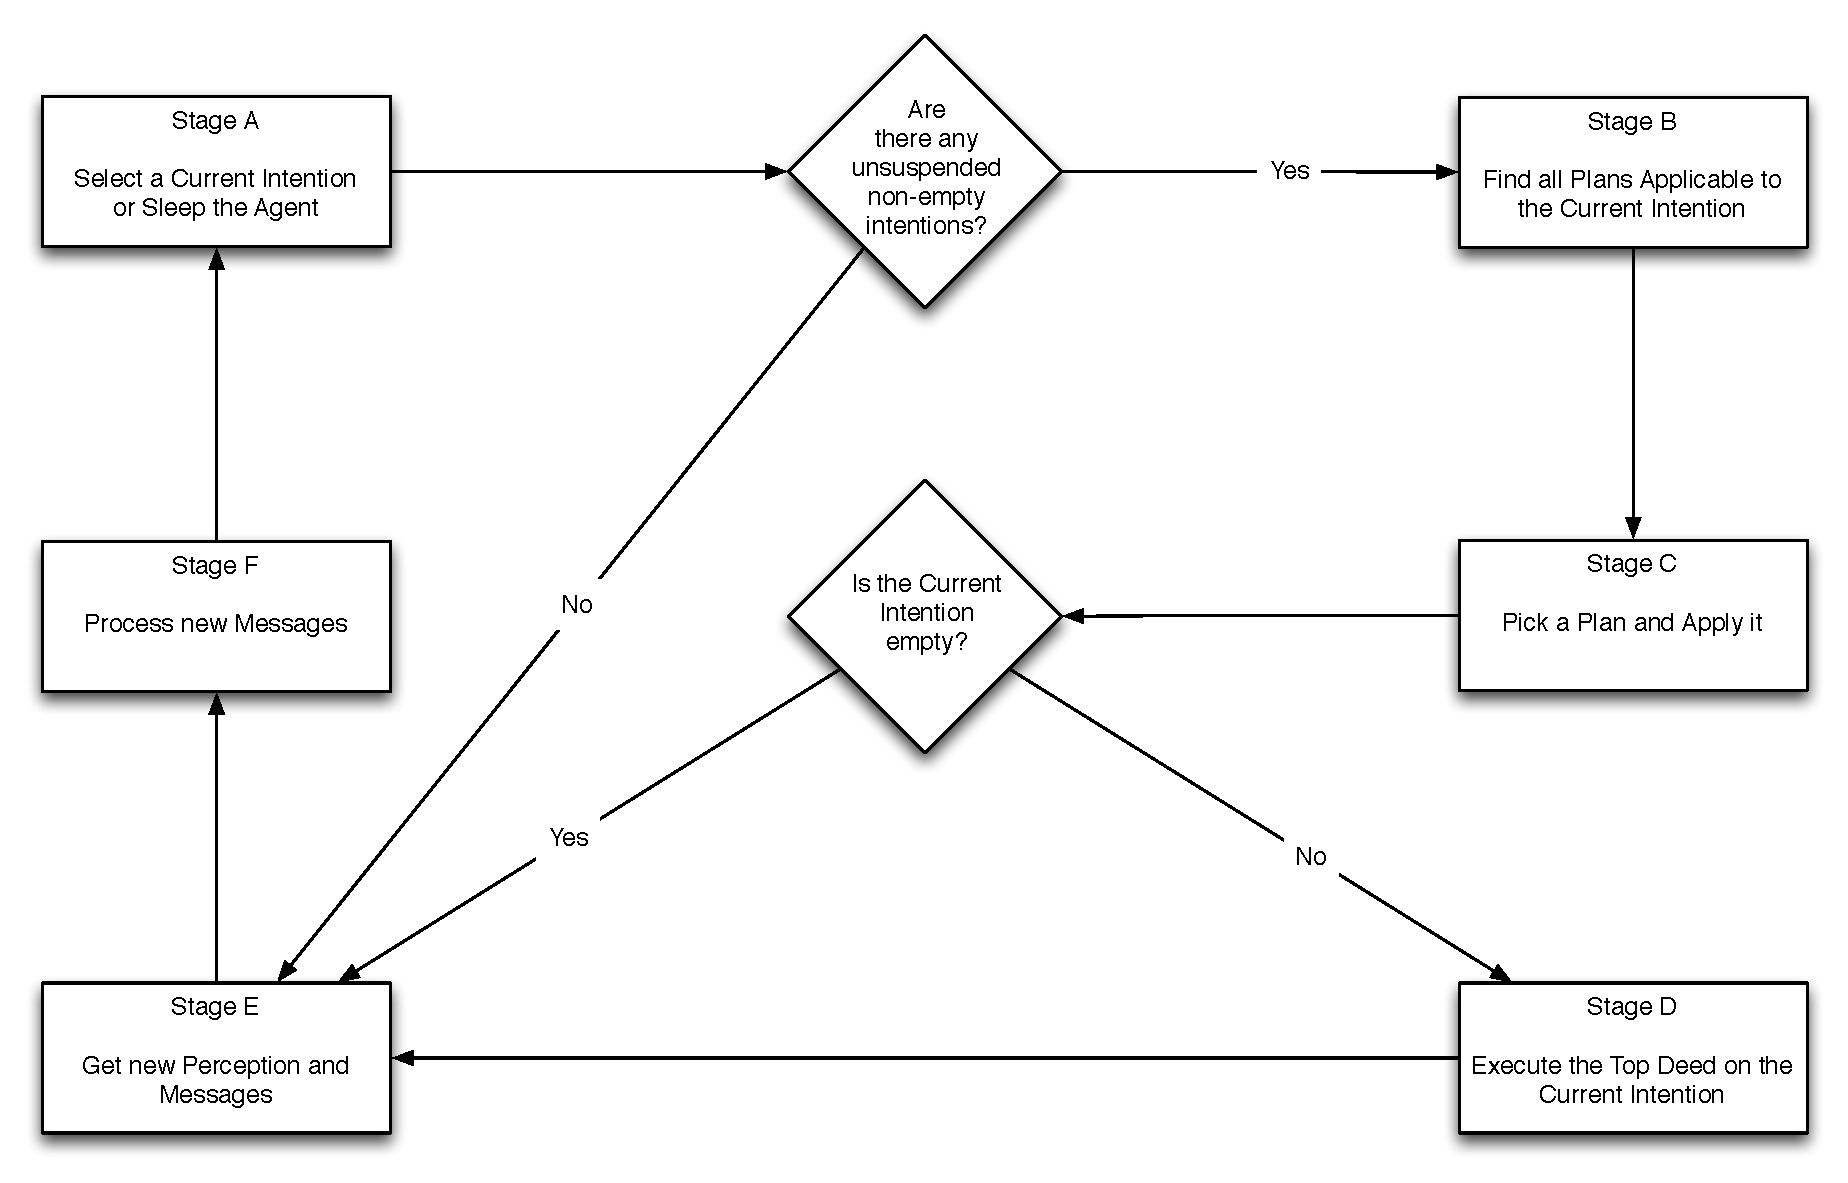
\includegraphics[width=\textwidth]{images/ReasoningCycle.pdf}
\caption{The \gwendolen\ Reasoning Cycle}
\label{fig:reasoning_cycle}
\end{figure}
\begin{description}
\item[Stage A]
A \gwendolen\ agent starts execution in stage A.  In this stage the
agent selects an intention to be the current
intention\index{intention}\index{intention!current}.  \gwendolen\ will
cycle through the set of intentions ignoring any that are
suspended\index{intention!suspension} until the current intention is
locked\index{intention!locking} in which case it will be reselected.
If there are no unsuspended intentions \gwendolen\ will sleep the
agent\index{sleeping}.  In multi-agent contexts this means the agent
will not do anything until \gwendolen\ detects that something has
changed which may mean the agent now has something to do.  In single
agent contexts the program stops when the agent sleeps.  At this stage
\gwendolen\ also cleans up any empty
intentions.\index{Gwendolen}\index{intention!empty} 
\item[Stage B]
The system generates all possible plans for the current intention - if
the intention has already been planned then these are simply to
continue processing the intention.  If the agent can't find a plan
then it deletes the intention unless it has been triggered by a goal
in which case it registers that there is a problem with the goal and
generates a
warning.\index{plan}\index{plan!generation}\index{goal}\index{goal!problem} 
\item[Stage C]
\gwendolen\ has a list of plans.  It selects the first one in the list
and applies it to the current
intention.\index{plan}\index{intention}\index{Gwendolen} 
\item[Stage D]
\gwendolen\ executes the top deed on the intention.  This might be
taking an action, adding or removing a goal, adding or removing a
belief, locking or unlocking the intention or suspending the intention
using ``wait
for''.\index{intention}\index{intention!execution}\index{deed}\index{deed!top} 
\item[Stage E]
\gwendolen\ requests that the agent's environment send it a list of
\emph{percepts} (things the agent can detect) and messages.  The
messages are stored for processing in the agent's inbox.  The percepts
are compared with the agent's beliefs.  If a percept is new then an
intention is created to add a belief corresponding to the percept.  If
a previous percept can no longer be perceived then an intention is
created to delete the
belief.\index{perception}\index{communication}\index{message} 
\item[Stage F]
The agent sorts though its inbox and converts the messages into new
intentions.\index{message!converted to intention}\index{Gwendolen} 
\end{description}

\begin{sloppypar}
The actual code for the reasoning cycle can be found in
\texttt{gwendolen.semantics.GwendolenRC}\index{GwendolenRC
  (class)}\index{reasoning cycle}.  Each of the various rules that can
be used in in a stage is a java class and they can all be found in the
package \texttt{ail.semantics.operationalrules}\index{operationalrules
  (package)}. 
\end{sloppypar}

\section{Using Java Debuggers to Debug \gwendolen\ programs}\index{debugging}\index{debugging!with a Java debugger}\index{Gwendolen!debugging}

Since the \gwendolen\ reasoning cycle\index{reasoning cycle} is
implemented in \java\ it is possible to use a \java\ debugger to debug
\gwendolen\ programs.  In particular it can be useful to use a
\java\ debugger to step through a \gwendolen\ program one stage of the
reasoning cycle at a time watching to see how the state of the agent
changes at each
stage.\index{Gwendolen}\index{debugging}\index{debugging!with a Java
  debugger}\index{Gwendolen!debugging} 

It is outside the scope of these tutorials to explain the use of
\java\ debuggers.  There are many out there and one is built into most
IDE's including Eclipse.\index{Java} 

In our experience it is particularly useful when debugging in this way
to place breakpoints in the
\java\ \texttt{ail.semantics.AILAgent}\index{AILAgent (class)} class
which is the generic class supporting agents in the Agent
Infrastructure Layer\index{AIL} (upon which \gwendolen\ is built).  In
particular \texttt{ail.semantics.AILAgent} has a method called
\texttt{reason}\index{AILAgent (class)!reason} which controls looping
through an agent's reasoning cycle\index{reasoning cycle}.  We
recommend placing such a break point either after \texttt{while(!
  RC.stopandcheck())} which is the top level loop through the
reasoning cycle or at \texttt{rule.apply(this)} which is the moment
that the outcome of a rule is calculated. 

\begin{sloppypar}
\paragraph{Exercise} Find a \java\ debugger (e.g., the one shipped
with Eclipse) and discover how to set breakpoints using the debugger.
Set a breakpoint at \texttt{rule.apply(this)} in the \texttt{reason()}
method in \texttt{ail.semantics.AILAgent} (you can find this in the
\texttt{src/classes/ail/semantics} directory).  Run one of your
programs with this breakpoint in place and see what happens and
experiment in seeing what information you can discover about the agent
state.\index{debugging!exercises}\index{AILAgent
  (class)}\index{AILAgent (class)!reason} 
\end{sloppypar}

\section{Programming Exercise}\index{Gwendolen}\index{Gwendolen!exercises}
This is a fairly major programming exercise using the
\gwendolen\ constructs you have already been introduced to.  As usual
a sample solution can be found in the \texttt{answers} subdirectory
for \texttt{tutorial7}. 

In \texttt{examples/gwendolen/tutorials/tutorial7} you will find a new
environment,
\texttt{SearchAndRescueDynamicEnv.java}\index{SearchAndRescueDynamicEnv
  (class)}.  This extends the previous search and rescue example so
that the environment may change with the agent directly taking any
action.  The following describes the environment. 

The environment consists of a 5x5 grid of squares.  The squares in the
grid are numbered from (0, 0) (bottom left) to (4, 4) (top right).  On
this grid are 
\begin{itemize}
\item Exactly four humans which may start in any square on the grid.
  Some of these humans may be {\bf injured}. 
\item Exactly one robot which starts in the bottom left corner of the grid.
\item Up to four buildings which may appear in any square on the grid.
\item Up to four bits of rubble which may appear in any square on the
  grid.  Any human on the same square as some rubble at the start is
  {\bf injured} and is hidden under the rubble. 
\end{itemize}

At any point the following may happen:
\begin{itemize}
\item A human who is not {\bf injured}, {\bf in a building}, or has
  been {\bf directed to leave} the area may move one square in any
  direction. 
\item A building may collapse into rubble.
\end{itemize}

The robot  has the following actions available to it:
\begin{description}
\item[back\_left] If possible the robot will move one square diagonally down the grid and to the left.  If not possible the robot will do nothing.
\item[back] If possible the robot will move one square down the grid.  If not possible the robot will do nothing.
\item[back\_right] If possible the robot will move one square diagonally down the grid and to the right.  If not possible the robot will do nothing.
\item[left] If possible the robot will move one square to the left.  If not possible the robot will do nothing.
\item[right] If possible the robot will move one square to the right.  If not possible the robot will do nothing.
\item[forward\_left] If possible the robot will move one square diagonally forward in the grid and to the left.  If not possible the robot will do nothing.
\item[forward] If possible the robot will move one square forward in the grid.  If not possible the robot will do nothing.
\item[forward\_right] If possible the robot will move one square diagonally forward in the grid and to the right.  If not possible the robot will do nothing.
\item[lift\_rubble] If the robot is not currently holding rubble then it will pick up one piece of rubble in the square revealing anything underneath it.
\item[drop\_rubble] If the robot is holding rubble then it will drop it in the current square, injuring and concealing any humans if they are in the square.
\item[assist\_human] If there is an injured human in the square then the robot treats them with first aid.  After this the human is not injured.
\item[direct\_humans] If there are any humans in the square then the robot tells them to leave the area immediately.
\item[check\_building] If there is a building in the square then the robot looks inside it to see if there is a human there.
\item[Other Actions] Other standard actions such as \texttt{print} and \texttt{do\_nothing} are also available.
\end{description}

The robot may perceive the following things:
\begin{description}
\item[holding\_rubble] perceived if the robot has rubble in its hands.
\item[rubble(X, Y)] perceived if the robot sees some rubble in square (X, Y).  The robot can see the square it is in and one square in each direction.
\item[building(X, Y)] perceived if the robot sees a building in square (X, Y).  The robot can see the square it is in and one square in each direction.
\item[injured\_human(X, Y)] perceived if the robot sees an injured human in square (X, Y).  The robot can see the square it is in and one square in each direction.
\item[uninjured\_human(X, Y)] perceived if the robot sees an uninjured human in square (X, Y).  The robot can see the square it is in and one square in each direction.
\end{description}

The following also hold true:
\begin{itemize}
\item If a human is {\bf in a building} when it collapses then they will be {\bf injured} and concealed by the rubble.
\item If a human is {\bf in a building} then the robot can not see them unless it checks the building.
\end{itemize}

Humans exhibit the following behaviour:
\begin{itemize}
\item {\bf injured} humans do not move.
\item {\bf directed} humans move diagonally down and left until they leave the grid.  They do not enter buildings.
\item If a human is not {\bf directed} and finds itself in a square with a building then it will enter the building and stay there.
\item Humans which are not {\bf injured}, {\bf directed} or {\bf in a building} will move at random around the grid.
\end{itemize}

\subsection{Recording and Replaying \ail\ Programs}\index{record random execution}\index{replay execution}
We will cover recording and replaying \ail\ programs in more detail in
a later tutorial.  However some of the challenges from this tutorial
will arise because of the difficulty in reproducing a specific
sequence of events in the environment.  In the \ail\ configuration
file you can put the line 

\begin{verbatim}
ajpf.record = true
\end{verbatim}

\index{ajpf.record}
This will record the sequence of events that occur in the environment
(and store them in a file called \texttt{record.txt} in the folder
\texttt{records}).  If you want to \emph{replay} the last recorded run
of the problem then replace 

\begin{verbatim}
ajpf.record = true
\end{verbatim}

with \index{ajpf.replay}

\begin{verbatim}
ajpf.replay = true
\end{verbatim}

\subsection{Exercise}
Write a \gwendolen\ program that will get the robot to search the grid
until all humans have been found, assisted if injured, and directed to
leave.\index{Gwendolen} 


  }

\section{Tutorial 8 --- Multi-Agent Systems and Communication}\index{Gwendolen}

{
  \let\section\subsection
  \let\subsection\subsubsection
  \let\subsubsection\paragraph
  
  \label{tutorial:gwendolen:communication}
This is the eighth in a series of tutorials on the use of the \gwendolen\ programming language.  This tutorial covers the use of communication in \gwendolen\ and also looks at setting up a multi-agent system.\index{Gwendolen}\index{communication}\index{multi-agent system}

Files for this tutorial can be found in the \texttt{mcapl} distribution in the directory 
\begin{quote}
\texttt{src/examples/gwendolen/tutorials/tutorial8}.
\end{quote}

\section{Pick Up Rubble (Again)}\index{Gwendolen}\index{example!pickuprubble}

\begin{sloppypar}
You will find a \gwendolen\ program in the tutorial directory called \texttt{simple\_mas.gwen}.  Its contents should look like Example~\ref{code:simple_mas}.\index{Gwendolen}\index{example!simple\_mas}
\end{sloppypar}
\begin{ourexample}
\label{code:simple_mas} \quad \\
\begin{lstlisting}[basicstyle=\sffamily,style=easslisting,language=Gwendolen]
GWENDOLEN

:name: lifter

:Initial Beliefs:

:Initial Goals:

goto55 [perform]

:Plans:

+!goto55 [perform] : {True} <- move_to(5, 5);

+rubble(5, 5): {True} <- lift_rubble;

+human(X, Y): {True} <- .send(medic, :perform, assist_human(X, Y));

:name: medic

:Initial Beliefs:

:Initial Goals:

:Plans:

+.received(:perform, G): {True} <- +!G [perform];

+!assist_human(X, Y) [perform] : {True} <- 
	move_to(X, Y),
	assist;
\end{lstlisting}
\end{ourexample}

This is very similar to the first program in tutorial 2.  However  there are now two agents, \texttt{lifter} and \texttt{medic}.  As in the program in tutorial 2, the lifter robot moves to square (5, 5) and lifts the rubble there.  However if he sees a human he performs a special kind of action which is a \emph{send action}.  This sends a message to the medic agent asking it to perform \texttt{assist\_human(X, Y)}.  When the medic receives a perform instruction it converts it into a perform goal and if it has a goal to assist a human it moves to their square and assists them.\index{Gwendolen}\index{example!lifterandmedic}\index{action}\index{action!send}

\begin{sloppypar}
You can run this program using \texttt{simple\_mas.ail}.  It uses a new environment \texttt{SearchAndRescueMASEnv.java} which is similar to \texttt{SearchAndRescueEnv.java}.
\end{sloppypar}\index{Gwendolen}\index{example!simple\_mas}\index{environment}\index{SearchAndRescueMASEnv (class)}

\subsection{Syntax}\index{Gwendolen}

A send action starts with the constant \texttt{.send}.  It then has three arguments:\index{action}\index{action!send}
\begin{enumerate}
\item The first is the name of the agent to whom the message is to be sent, \index{message}\index{message!recipient}
\item the second is a performative, and \index{performative}\index{message!performative}
\item the last is a logical term.  \index{message!logical content}
\end{enumerate}\index{Gwendolen}
The performative\index{performative} can be one of \texttt{:tell}, \texttt{:perform} or \texttt{:achieve}.  \gwendolen\ attaches no particular meaning to these performatives but they are often used to tell an agent to believe something, ask an agent to adopt a perform goal or ask an agent to adopt an achieve goal.\index{:tell}\index{:perform}\index{:achieve}

\begin{sloppypar}
When a message is received \gwendolen\ turns it into an event: \texttt{.received(P,~F)} were \texttt{P} is the performative and \texttt{F} is the logical term.  Since many \gwendolen\ programs interpret \texttt{:tell}, \texttt{:perform} and \texttt{:achieve} as described above, they often include the following three plans \index{Gwendolen}\index{plan}\index{message}\index{message!converted to event}\index{message!performative}\index{message!logical content}
\end{sloppypar}
\begin{verbatim}
+.received(:tell, B): {True} <- +B;
+.received(:perform, G): {True} <- +!G [perform];
+.received(:achieve, G): {True} <- +!G [achieve];
\end{verbatim}
which embody that interpretation.  However many programs instead choose only to handle certain performatives (e.g., only \texttt{:tell} messages) or only certain message contents, (e.g., \texttt{.received(:perform, assist\_human(X, Y))} only handles messages asking the agent to perform \texttt{assist\_human(X, Y)} for some \texttt{X} and \texttt{Y}).\index{Gwendolen!message handling}\index{:tell}\index{:perform}\index{:achieve}

\subsection{Exercise}\index{Gwendolen!exercises}
Amend the \texttt{simple\_mas} program so that, instead of sending a perform message, the lifter agent sends a tell message and the medic reacts to the new belief, instead of the new goal.\index{example!simple\_mas}\index{message}

NB. It is important, for using the \texttt{SearchAndRescueMASEnv.java} environment that the lifting agent be called \texttt{lifter} and the medic agent be called \texttt{medic}.\index{example!lifterandmedic}\index{SearchAndRescueMASEnv (class)}\index{Gwendolen}

As usual sample solutions to all the exercises can be found in the \texttt{answers} directory for \texttt{tutorial8}.

\section{Recording and Replaying \ail\ Programs}\index{record random execution}\index{replay execution}
Now there is more than one agent in the system, you will observe that there are several paths through the program.  These depend upon which agent acts when.  Sometimes the \texttt{lifter} agent will go first (moving to (5, 5)) and sometimes the \texttt{medic} agent will go first (sleeping).\index{sleeping}\index{Gwendolen}\index{scheduler}

When debugging a multi-agent program you sometimes want to replay the exact sequence of events that occurred in the  problem run.  To do this you first need to record the sequence.  You can get an \ail\ program to record its sequence of choices (in this case choices about which agent goes first) by adding the line\index{debugging!multi-agent program}

\begin{verbatim}
ajpf.record = true
\end{verbatim}

\index{ajpf.record}To the program's \ail\ configuration file.  By default this records the current path through the program in a file called \texttt{record.txt} in the directory, \texttt{records} of the \mcapl\ distribution.  You can change the file using \texttt{ajpf.replay.file =}.  There is an example of this in the configuration file \texttt{simple\_mas\_record.ail} in the tutorial directory.\index{Gwendolen}\index{ajpf.replay.file}\index{example!simple\_mas}

When you want to play back a record then include 

\begin{verbatim}
ajpf.replay = true
\end{verbatim}

\index{ajpf.replay}In the program's \ail\ configuration file.  Again, by default, this will replay the sequence from \texttt{record.txt}, but will use a different file if \texttt{ajpf.replay.file = } is set.  The configuration file \texttt{simple\_mas\_replay.ail} is set up to replay runs generated by \texttt{simple\_mas\_record.ail}\index{example!simple\_mas}

\section{Two Ways to Create a Multi-Agent System}\index{Gwendolen}\index{multi-agent system}

\begin{sloppypar}
In the previous example we put all the agents in a multi-agent system in one file.  However you often want to separate out your agents into different files, one for each agent.  This is easy to do in the \ail.  You write each agent as you normally would in a separate file.  Then in the \texttt{.ail} file for running the system instead of using \texttt{mas.file}\index{mas.file} you use \texttt{mas.agent.1.file}\index{mas.agent.1.file} (for the file containing agent one), \texttt{mas.agent.2.file} etc.  Similarly instead of using a MAS builder you link to individual agent builders.  \gwendolen's agent builder is \texttt{gwendolen.GwendolenAgentBuilder}\index{GwendolenAgentBuilder (class)} -- so you use 
\end{sloppypar}
\begin{center}
\texttt{mas.agent.1.builder = gwendolen.GwendolenAgentBuilder} 
\end{center}
etc., for each agent rather than \index{mas.agent.1.builder}
\begin{center}
\texttt{mas.builder = gwendolen.GwendolenMASBuilder}.
\end{center}\index{GwendolenMASBuilder (class)}

\subsection{Exercise}\index{Gwendolen!exercises}\index{Gwendolen}
Convert \texttt{simple\_mas.gwen} into a system consisting of two agents in different files.  NB.  You will need to make sure both agent files start with the declaration \texttt{GWENDOLEN} for the language the agent is programmed in.\index{example!simple\_mas}

\section{Duplicating an Agent}

Sometimes you want to create a multi-agent system in which all agents behave identically.  Ideally you would like to use the same agent code file for all these agents and just give them different names in the multi-agent system.\index{agent!renaming}

You can do this using files and builders, as above, with the addition of a \texttt{name} setting.  So, for instance, \texttt{mas.agent.3.name = nurse}\index{mas.agent.1.name} sets the name of agent 3 to \texttt{nurse} instead of whatever is given in the agent file.\index{Gwendolen}

\subsection{Exercise}\index{Gwendolen}\index{Gwendolen!exercises}
Adapt the system from exercise 2 by creating a new lifter agent that visits first square (5, 5) and summons the medic to assist the human there and, after that, visits square (3, 4) and summons a nurse to assist the human there.  The medic and the nurse should both use the medic agent code file you developed for exercise 2.  Give one of these agent's the name \texttt{nurse} in the \texttt{.ail} file.


  }

\section{Tutorial 9 --- Default built-in actions: Strings and Arithmetic}\index{Gwendolen}

{
  \let\section\subsection
  \let\subsection\subsubsection
  \let\subsubsection\paragraph
  
  
This is the ninth in a series of tutorials on the use of the \gwendolen\ programming language\index{Gwendolen}.  This tutorial covers a few final elements of \gwendolen\ and the actions\index{action} that come with the Default Environment\index{environment!default}.  It is important to note that if a \gwendolen\ agent \emph{isn't} operating in some environment sub-classed from \texttt{DefaultEnvironment}\index{DefaultEnvironment (class)} then there is no guarantee that these actions will be available.

Files for this tutorial can be found in the \texttt{mcapl} distribution in the directory 
\begin{quote}
\texttt{src/examples/gwendolen/tutorials/tutorial9}.
\end{quote}

\section{String Handling}\index{Gwendolen}\index{strings}\index{action}

In the tutorial directory you will find a program called \texttt{strings.gwen}.  It's contents should look like Example~\ref{code:strings}
\begin{ourexample}
\label{code:strings} \quad \\
\begin{lstlisting}[basicstyle=\sffamily,style=easslisting,language=Gwendolen]
:name: strings

:Initial Beliefs:

string1("hello")
string2(" ")
string3("world")

:Initial Goals:

print_string [perform]

:Plans:

+! print_string [perform] : {True} <-
	print("hello world");
\end{lstlisting}
\end{ourexample}\index{example!hello\_world}
If you run this program you will see that it prints out \texttt{hello world}.  Here ``print'' is an action\index{action}\index{action!print} which is implemented in \texttt{DefaultEnvironment}\index{DefaultEnvironment (class)}\index{Gwendolen}

\subsection{Built-in String Actions}\index{action}
If you look at \texttt{strings.ail} you will see that you are using \ail's \texttt{DefaultEnvironment}\index{DefaultEnvironment (class)}\index{strings} class.  Most \gwendolen\ environments are based on the default environment and this means they all support a set of standard actions that come with the Default Environment.  The built-in actions for strings are:
\begin{description}\index{action}\index{action!in DefaultEnvironment}\index{action!toString}\index{action!append}
\item[toString(T, S)] This will take any term, \lstinline{T}, that you are passing around your program and unify the variable, \lstinline{S}, to that term.
\item[append(S1, S2, S3)]  This takes two strings, \lstinline{S1} and \lstinline{S2} and unifies, \lstinline{S3}, to the concatenation of those two strings.  So, for instance, \lstinline{append(``gwen",``dolen",S)} will unify \lstinline{S} to \lstinline{gwendolen}.
\end{description}\index{Gwendolen}

\subsection{Exercise}\index{Gwendolen!exercises}\index{action}
You will notice that \texttt{strings.gwen} contains three beliefs about strings.  Adapt the program so that instead of printing out \texttt{hello world} directly, it instead uses \lstinline{append} to join the three strings together to print out the message.\index{action!append}

\paragraph{Hint.} You will need to use \lstinline{append} twice.\index{Gwendolen}

As usual you can find sample solutions in the \texttt{answers} directory.

\section{Arithmetic}\index{Gwendolen}\index{action!arithmetic}\index{action}

\gwendolen\ can use numbers as terms but it is both fiddly and inefficient to program up arithmetic operations using Reasoning Rules.  As a result the Default environment has four simple actions for manipulating numbers.\index{Gwendolen}\index{DefaultEnvironment (class)}\index{action!in DefaultEnvironment}

\begin{description}
\item[sum(X, Y, Z)] This unifies \lstinline{Z} to the sum of \lstinline{X} and \lstinline{Y}.\index{action!sum}
\item[minus(X, Y, Z)] This takes \lstinline{Y} away from \lstinline{X} and unifies \lstinline{Z} to the result.\index{action!minus}
\item[div(X, Y, Z)] This divides \lstinline{X} by \lstinline{Y} and unifies \lstinline{Z} to the result.\index{action!div}
\item[times(X, Y, Z)] This multiplies \lstinline{X} by \lstinline{Y} and unifies \lstinline{Z} to the result.\index{action!times}
\end{description}\index{action!in DefaultEnvironment}\index{action!arithmetic}\index{Gwendolen}

\subsection{Exercise}\index{Gwendolen}\index{Gwendolen!exercises}\index{action}
In the tutorial directory you will find a partial program, \texttt{arithmetic\_shell.gwen}.  This is shown in Example~\ref{code:arithmetic}

\begin{ourexample}
\label{code:arithmetic} \quad \\
\begin{lstlisting}[basicstyle=\sffamily,style=easslisting,language=Gwendolen]
GWENDOLEN

:name: arithmetic

:Initial Beliefs:

:Initial Goals:

do_maths [perform]

:Plans:
	
+! do_maths[perform] : {True} <-
	+! do_sum [perform],
	+! do_minus [perform],
	+! do_div [perform],
	+! do_mult [perform];
\end{lstlisting}
\end{ourexample}\index{example!arithmetic}

Implement the four missing plans so that\index{Gwendolen}\index{arithmetic}
\begin{itemize}
\item \lstinline{do_sum} adds two numbers and prints out the result as, for instance, \texttt{The Sum of 1 and 5 is 6}.  You will need to use \texttt{toString} and \texttt{append} to generate the string you want.
\item \lstinline{do_minus} subtracts two numbers and prints out the result as, for instance, \texttt{5.5. take 3.2. is 2.3}.
\item \lstinline{do_div} divides one number by another and prints out the result as, for instance, \texttt{7 divided by 2 is 3.5}
\item \lstinline{do_mult} multiplies two numbers and prints out the result as, for instance, \texttt{100 times 2.5 is 250}.
\end{itemize}

\section{Using Equations in Plan Guards}\index{Gwendolen}\index{inequalities}
Once you are using numbers in your program you quickly get to situations where you want to use equations in plan guards\index{plan}\index{plan!guard}\index{inequalities!in plan guard}.  \gwendolen\ has some limited support for this.  It can't perform arithmetic in the guards of plans, but it can compare numbers using \texttt{<} (less than) and \texttt{==} (equals).

\subsection{Exercise}\index{Gwendolen}\index{Gwendolen!exercise}\index{example!inequalities}
In the tutorial directory you will find a partial program, \texttt{equation\_shell.gwen}.  This is shown in Example~\ref{code:equation}

\begin{ourexample}
\label{code:equation} \quad \\
\begin{lstlisting}[basicstyle=\sffamily,style=easslisting,language=Gwendolen]
GWENDOLEN

:name: equation

:Initial Beliefs:

number1(3)
number2(5)
number3(4.8)
number4(3)

:Initial Goals:

compare_numbers [perform]

:Plans:

+! compare_numbers [perform] : {B number1(N1), B number2(N2), 
                                B number3(N3), B number4(N4)} <-
	+!compare(N1, N2) [perform],
	+!compare(N1, N3) [perform],
	+!compare(N1, N4) [perform],
	+!compare(N2, N3) [perform],
	+!compare(N2, N4) [perform],
	+!compare(N3, N4) [perform];
\end{lstlisting}
\end{ourexample}

Complete this program by implementing plans for the goal, \lstinline{compare(N1, N2)}, so that the program prints out the following output.\index{Gwendolen}

\begin{verbatim}
3 is less than 5
3 is less than 4.8
3 is equal to 3
4.8 is less than 5
3 is less than 5
3 is less than 4.8
\end{verbatim}

\section{Print Actions}\index{action!print}\index{Gwendolen}\index{DefaultEnvironment (class)}\index{action!in DefaultEnvironment}\index{action}

\gwendolen's default environment has three print actions.\index{action!print}
\begin{description}
\item[print(X)] you have already encountered and prints out the term, \lstinline{X}.\index{action!print}\index{action}
\item[printagentstate] prints the current state of the agent to standard error.\index{action!printagentstate}
\item[printstate] prints the current state of the agent to standard out.\index{action!printstate}
\end{description}
Clearly \lstinline{printagentstate} and \lstinline{printstate} are virtually identical.  They are mostly of use when debugging\index{debugging}\index{debugging!program}\index{debugging!agent state} and generally either can be used, but in certain situations you may have a preference about which output channel you want to use.\index{Gwendolen}\index{action}

\subsection{Exercise}\index{Gwendolen!exercises}
Experiment inserting \lstinline{printagentstate} and \lstinline{printstate} into one of your existing programs.


  }

\section{The Property Specification Language and its Relation to \gwendolen\ Programs}\index{Gwendolen}

{
  \let\section\subsection
  \let\subsection\subsubsection
  \let\subsubsection\paragraph
  
  \section{Implementation of BDI Modalities in \gwendolen}
\label{s:impl_bdi}

In \gwendolen\ the BDI modalities of the \ajpf\ property specification language are implemented as follows.

\begin{itemize}
\item $\lbelief{\AILagent}{f}$.  An agent, $\AILagent$, believes the formula, $f$, if $f$ appears in its belief base or is deducible from its goal base using its reasoning rules.
\item $\lgoal{\AILagent}{f}$.  An agent, $\AILagent$, has a goal $f$, if $f$ is a goal that appears in the agent's goal base.
\item $\lintention{\AILagent}{f}$.  An agent, $\AILagent$, has an intention $f$, if $f$ is a goal in the goal base a plan has been selected to achieve or perform the goal.
\item $\lintendtodo{\AILagent}{f}$.  An agent, $\AILagent$, intends to do $f$, if $f$ is an action that appears in the deed stack of some intention.
\end{itemize}

\subsection{Intending to Send a Message}
\gwendolen\ uses a special syntax for send actions (\texttt{.send(ag, :tell, c)}) which is not recognised by the property specification language.  If you want to check that a \gwendolen\ agent intends to send a messsage then you need to use the syntax \texttt{send(agname, number, c)} where \texttt{agname} is the name of the recipient, \texttt{number} is
\begin{description}
\item[1] For \texttt{:tell},
\item[2] For \texttt{:perform},
\item[3] For \texttt{:achieve}
\end{description}
and \texttt{c} is the content of the message.


  }
